
% Module 4: starts Denoising autoencoders (Slide 28 to 39)
\begin{frame}
    \myheading{Module 7.4: Denoising Autoencoders }
\end{frame}

\begin{frame}
    %\begin{overlayarea}{\textwidth}{\textheight}
        \begin{columns}
        \column{0.5\textwidth}
        \begin{overlayarea}{\textwidth}{\textheight}
        % \tikzstyle{input_neuron}=[circle,draw=red!50,fill=red!10,thick,minimum size=6mm]
\tikzstyle{hidden_neuron}=[circle,draw=blue!50,fill=cyan!10,thick,minimum size=6mm]
\tikzstyle{output_neuron}=[circle,draw=green!50,fill=green!10,thick,minimum size=6mm]
\tikzstyle{cpy_neuron}=[circle,draw=red!50,fill=red!50,thick,minimum size=6mm]
\tikzstyle{input}=[circle,draw=black!50,fill=black!20,thick,minimum size=6mm]

\begin{center}
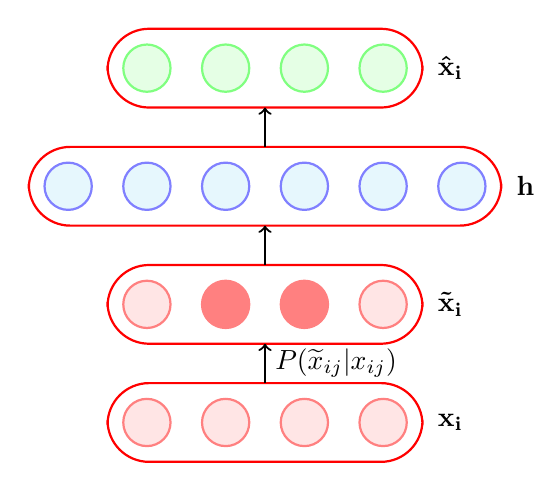
\begin{tikzpicture}

\node [input_neuron] (neuron001) at (8.5,3) {};
\node [input_neuron] (neuron002) at (9.5,3){};
\node [input_neuron] (neuron003) at (10.5,3) {};
\node [input_neuron] (neuron004) at (11.5,3) {};

\node [input_neuron] (neuron01) at (8.5,4.5) {};
\node [cpy_neuron] (neuron02) at (9.5,4.5){};
\node [cpy_neuron] (neuron03) at (10.5,4.5) {};
\node [input_neuron] (neuron04) at (11.5,4.5) {};

\node [hidden_neuron] (neuron51) at (7.5,6) {} ;
\node [hidden_neuron] (neuron52) at (8.5,6)  {};
\node [hidden_neuron] (neuron53) at (9.5,6)  {};
\node [hidden_neuron] (neuron54) at (10.5,6)  {};
\node [hidden_neuron] (neuron55) at (11.5,6)  {};
\node [hidden_neuron] (neuron56) at (12.5,6)  {};

\node [output_neuron] (neuron11) at (8.5,7.5)  {};
\node [output_neuron] (neuron12) at (9.5,7.5)  {};
\node [output_neuron] (neuron13) at (10.5,7.5)  {};
\node [output_neuron] (neuron14) at (11.5,7.5)  {};

\node[text width=0.01cm] at (12.2,3) {$\mathbf{\textbf{x}_i}$};
\node[text width=0.01cm] at (12.2,4.5) {$\mathbf{\tilde{\textbf{x}}_i}$};
\node[text width=0.01cm] at (13.2,6) {$\mathbf{h}$};
\node[text width=0.01cm] at (12.2,7.5) {$\mathbf{\hat{x}_{i}}$};

\draw[red!100,thick,solid,rounded corners=15pt] (8,2.5) rectangle (12,3.5);
\draw[red!100,thick,solid,rounded corners=15pt] (8,4) rectangle (12,5);
\draw[red!100,thick,solid,rounded corners=15pt] (7,5.5) rectangle (13,6.5);
\draw[red!100,thick,solid,rounded corners=15pt] (8,7) rectangle (12,8);

\draw[thick,->] (10,3.5) -- (10,4) node [pos=0.5,right] {$P(\widetilde{x}_{ij}|x_{ij})$};

\draw[thick,->] (10,5) -- (10,5.5);

\draw[thick,->] (10,6.5) -- (10,7);

\end{tikzpicture}
\end{center}
        \vspace{10pt}
        \tikzstyle{input_neuron}=[circle,draw=red!50,fill=red!10,thick,minimum size=6mm]
\tikzstyle{hidden_neuron}=[circle,draw=blue!50,fill=cyan!10,thick,minimum size=6mm]
\tikzstyle{output_neuron}=[circle,draw=green!50,fill=green!10,thick,minimum size=6mm]
\tikzstyle{cpy_neuron}=[circle,draw=red!50,fill=red!50,thick,minimum size=6mm]
\tikzstyle{input}=[circle,draw=black!50,fill=black!20,thick,minimum size=6mm]

\begin{center}
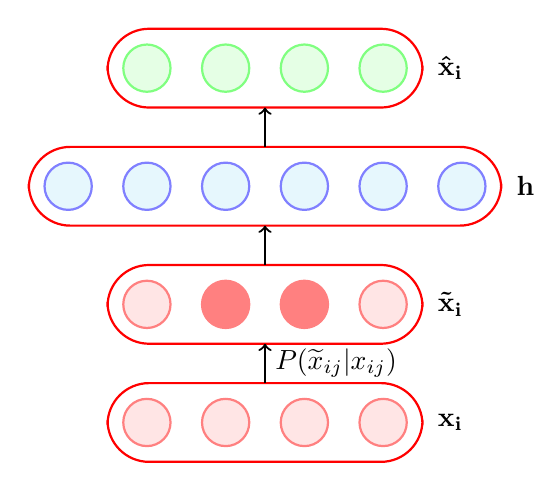
\begin{tikzpicture}

\node [input_neuron] (neuron001) at (8.5,3) {};
\node [input_neuron] (neuron002) at (9.5,3){};
\node [input_neuron] (neuron003) at (10.5,3) {};
\node [input_neuron] (neuron004) at (11.5,3) {};

\node [input_neuron] (neuron01) at (8.5,4.5) {};
\node [cpy_neuron] (neuron02) at (9.5,4.5){};
\node [cpy_neuron] (neuron03) at (10.5,4.5) {};
\node [input_neuron] (neuron04) at (11.5,4.5) {};

\node [hidden_neuron] (neuron51) at (7.5,6) {} ;
\node [hidden_neuron] (neuron52) at (8.5,6)  {};
\node [hidden_neuron] (neuron53) at (9.5,6)  {};
\node [hidden_neuron] (neuron54) at (10.5,6)  {};
\node [hidden_neuron] (neuron55) at (11.5,6)  {};
\node [hidden_neuron] (neuron56) at (12.5,6)  {};

\node [output_neuron] (neuron11) at (8.5,7.5)  {};
\node [output_neuron] (neuron12) at (9.5,7.5)  {};
\node [output_neuron] (neuron13) at (10.5,7.5)  {};
\node [output_neuron] (neuron14) at (11.5,7.5)  {};

\node[text width=0.01cm] at (12.2,3) {$\mathbf{\textbf{x}_i}$};
\node[text width=0.01cm] at (12.2,4.5) {$\mathbf{\tilde{\textbf{x}}_i}$};
\node[text width=0.01cm] at (13.2,6) {$\mathbf{h}$};
\node[text width=0.01cm] at (12.2,7.5) {$\mathbf{\hat{x}_{i}}$};

\draw[red!100,thick,solid,rounded corners=15pt] (8,2.5) rectangle (12,3.5);
\draw[red!100,thick,solid,rounded corners=15pt] (8,4) rectangle (12,5);
\draw[red!100,thick,solid,rounded corners=15pt] (7,5.5) rectangle (13,6.5);
\draw[red!100,thick,solid,rounded corners=15pt] (8,7) rectangle (12,8);

\draw[thick,->] (10,3.5) -- (10,4) node [pos=0.5,right] {$P(\widetilde{x}_{ij}|x_{ij})$};

\draw[thick,->] (10,5) -- (10,5.5);

\draw[thick,->] (10,6.5) -- (10,7);

\end{tikzpicture}
\end{center}
        \end{overlayarea}
        \column{0.5\textwidth}
        \begin{overlayarea}{\textwidth}{\textheight}
                \begin{itemize}\justifying
            \item<1-> A denoising encoder simply corrupts the input data using a probabilistic process ($P(\widetilde{x}_{ij} | x_{ij})$) before feeding it to the network
            \item<2-> A simple $P(\widetilde{x}_{ij} | x_{ij})$ used in practice is the following
            \begin{align*}
                \onslide<3->{P(\widetilde{x}_{ij} = 0 | x_{ij}) &= q }\\ 
                \onslide<4->{P(\widetilde{x}_{ij} = x_{ij} | x_{ij}) &= 1-q}
            \end{align*}
            \item<5-> In other words, with probability $q$ the input is flipped to 0 and with probability $(1-q)$ it is retained as it is 
        \end{itemize}
        \end{overlayarea}
        \end{columns}
    %\end{overlayarea}
\end{frame}

\begin{frame}
    %\begin{overlayarea}{\textwidth}{\textheight}

                \begin{columns}
        \column{0.5\textwidth}
        \begin{overlayarea}{\textwidth}{\textheight}
        % \tikzstyle{input_neuron}=[circle,draw=red!50,fill=red!10,thick,minimum size=6mm]
\tikzstyle{hidden_neuron}=[circle,draw=blue!50,fill=cyan!10,thick,minimum size=6mm]
\tikzstyle{output_neuron}=[circle,draw=green!50,fill=green!10,thick,minimum size=6mm]
\tikzstyle{cpy_neuron}=[circle,draw=red!50,fill=red!50,thick,minimum size=6mm]
\tikzstyle{input}=[circle,draw=black!50,fill=black!20,thick,minimum size=6mm]

\begin{center}
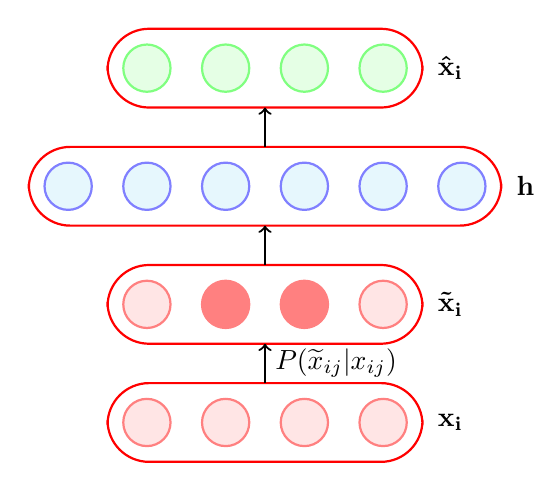
\begin{tikzpicture}

\node [input_neuron] (neuron001) at (8.5,3) {};
\node [input_neuron] (neuron002) at (9.5,3){};
\node [input_neuron] (neuron003) at (10.5,3) {};
\node [input_neuron] (neuron004) at (11.5,3) {};

\node [input_neuron] (neuron01) at (8.5,4.5) {};
\node [cpy_neuron] (neuron02) at (9.5,4.5){};
\node [cpy_neuron] (neuron03) at (10.5,4.5) {};
\node [input_neuron] (neuron04) at (11.5,4.5) {};

\node [hidden_neuron] (neuron51) at (7.5,6) {} ;
\node [hidden_neuron] (neuron52) at (8.5,6)  {};
\node [hidden_neuron] (neuron53) at (9.5,6)  {};
\node [hidden_neuron] (neuron54) at (10.5,6)  {};
\node [hidden_neuron] (neuron55) at (11.5,6)  {};
\node [hidden_neuron] (neuron56) at (12.5,6)  {};

\node [output_neuron] (neuron11) at (8.5,7.5)  {};
\node [output_neuron] (neuron12) at (9.5,7.5)  {};
\node [output_neuron] (neuron13) at (10.5,7.5)  {};
\node [output_neuron] (neuron14) at (11.5,7.5)  {};

\node[text width=0.01cm] at (12.2,3) {$\mathbf{\textbf{x}_i}$};
\node[text width=0.01cm] at (12.2,4.5) {$\mathbf{\tilde{\textbf{x}}_i}$};
\node[text width=0.01cm] at (13.2,6) {$\mathbf{h}$};
\node[text width=0.01cm] at (12.2,7.5) {$\mathbf{\hat{x}_{i}}$};

\draw[red!100,thick,solid,rounded corners=15pt] (8,2.5) rectangle (12,3.5);
\draw[red!100,thick,solid,rounded corners=15pt] (8,4) rectangle (12,5);
\draw[red!100,thick,solid,rounded corners=15pt] (7,5.5) rectangle (13,6.5);
\draw[red!100,thick,solid,rounded corners=15pt] (8,7) rectangle (12,8);

\draw[thick,->] (10,3.5) -- (10,4) node [pos=0.5,right] {$P(\widetilde{x}_{ij}|x_{ij})$};

\draw[thick,->] (10,5) -- (10,5.5);

\draw[thick,->] (10,6.5) -- (10,7);

\end{tikzpicture}
\end{center}
        \vspace{10pt}
        \tikzstyle{input_neuron}=[circle,draw=red!50,fill=red!10,thick,minimum size=6mm]
\tikzstyle{hidden_neuron}=[circle,draw=blue!50,fill=cyan!10,thick,minimum size=6mm]
\tikzstyle{output_neuron}=[circle,draw=green!50,fill=green!10,thick,minimum size=6mm]
\tikzstyle{cpy_neuron}=[circle,draw=red!50,fill=red!50,thick,minimum size=6mm]
\tikzstyle{input}=[circle,draw=black!50,fill=black!20,thick,minimum size=6mm]

\begin{center}
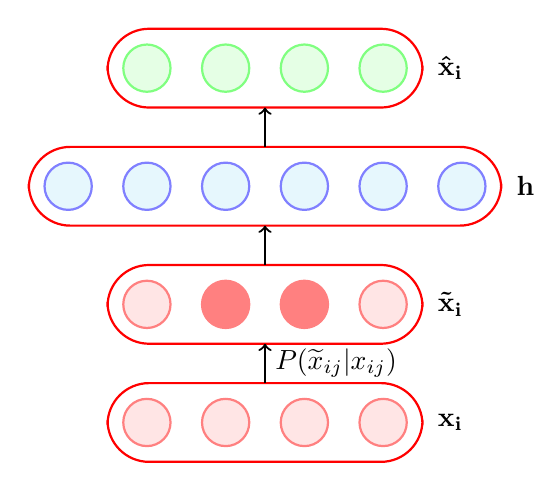
\begin{tikzpicture}

\node [input_neuron] (neuron001) at (8.5,3) {};
\node [input_neuron] (neuron002) at (9.5,3){};
\node [input_neuron] (neuron003) at (10.5,3) {};
\node [input_neuron] (neuron004) at (11.5,3) {};

\node [input_neuron] (neuron01) at (8.5,4.5) {};
\node [cpy_neuron] (neuron02) at (9.5,4.5){};
\node [cpy_neuron] (neuron03) at (10.5,4.5) {};
\node [input_neuron] (neuron04) at (11.5,4.5) {};

\node [hidden_neuron] (neuron51) at (7.5,6) {} ;
\node [hidden_neuron] (neuron52) at (8.5,6)  {};
\node [hidden_neuron] (neuron53) at (9.5,6)  {};
\node [hidden_neuron] (neuron54) at (10.5,6)  {};
\node [hidden_neuron] (neuron55) at (11.5,6)  {};
\node [hidden_neuron] (neuron56) at (12.5,6)  {};

\node [output_neuron] (neuron11) at (8.5,7.5)  {};
\node [output_neuron] (neuron12) at (9.5,7.5)  {};
\node [output_neuron] (neuron13) at (10.5,7.5)  {};
\node [output_neuron] (neuron14) at (11.5,7.5)  {};

\node[text width=0.01cm] at (12.2,3) {$\mathbf{\textbf{x}_i}$};
\node[text width=0.01cm] at (12.2,4.5) {$\mathbf{\tilde{\textbf{x}}_i}$};
\node[text width=0.01cm] at (13.2,6) {$\mathbf{h}$};
\node[text width=0.01cm] at (12.2,7.5) {$\mathbf{\hat{x}_{i}}$};

\draw[red!100,thick,solid,rounded corners=15pt] (8,2.5) rectangle (12,3.5);
\draw[red!100,thick,solid,rounded corners=15pt] (8,4) rectangle (12,5);
\draw[red!100,thick,solid,rounded corners=15pt] (7,5.5) rectangle (13,6.5);
\draw[red!100,thick,solid,rounded corners=15pt] (8,7) rectangle (12,8);

\draw[thick,->] (10,3.5) -- (10,4) node [pos=0.5,right] {$P(\widetilde{x}_{ij}|x_{ij})$};

\draw[thick,->] (10,5) -- (10,5.5);

\draw[thick,->] (10,6.5) -- (10,7);

\end{tikzpicture}
\end{center}
        \vspace{-0.2in}
        \onslide<5->{\normalsize{For example, it will have to learn to reconstruct a corrupted $x_{ij}$ correctly by relying on its interactions with other elements of $\textbf{x}_{i}$}}
        \end{overlayarea}
        \column{0.5\textwidth}
        \begin{overlayarea}{\textwidth}{\textheight}
        \begin{itemize}\justifying
            \item<1-> How does this help ?
            \item<2-> This helps because the objective is still to reconstruct the original (uncorrupted) $\textbf{x}_{i}$ 
            \vspace{-0.1in}
            \begin{align*}
                \underset{\theta}{\arg \min} \frac{1}{m}\sum\limits_{i=1}^m\sum\limits_{j=1}^n(\hat{x}_{ij}-x_{ij})^2
                % Expand loss function from module 3
            \end{align*}
            
            \vspace{-0.1in}
            \item<3-> It no longer makes sense for the model to copy the corrupted $\widetilde{\textbf{x}_i}$ into $h(\widetilde{\textbf{x}_i})$ and then into $\hat{\textbf{x}}_{i}$ (the objective function will not be minimized by doing so)
            \item<4-> Instead the model will now have to capture the characteristics of the data correctly.
        \end{itemize}
        \end{overlayarea}
        \end{columns}
    %\end{overlayarea}
\end{frame}

\begin{frame}
    \begin{block}{}
     We will now see a practical application in which AEs are used and then compare Denoising Autoencoders with regular autoencoders
    \end{block}
\end{frame}

\begin{frame}  
\begin{columns}
    \column{0.4\textwidth}

    \begin{overlayarea}{\textwidth}{\textheight}
        \vspace{0.2in}
    \textbf{\large{Task: Hand-written digit recognition}}
        \begin{figure}
            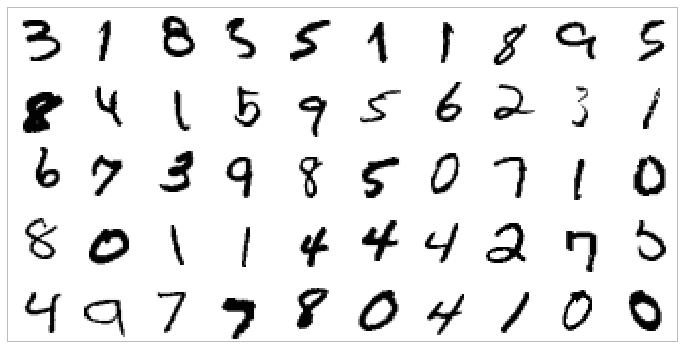
\includegraphics[scale= 0.25]{images/mnist.png}
        \caption{MNIST Data}
    \end{figure}
    \end{overlayarea}

    \column{0.6\textwidth}
    \begin{overlayarea}{\textwidth}{\textheight}

        \begin{figure}
            %
\tikzstyle{input_neuron}=[circle,draw=red!50,fill=red!10,thick,minimum size=6mm]
\tikzstyle{hidden_neuron}=[circle,draw=blue!50,fill=cyan!10,thick,minimum size=6mm]
\tikzstyle{output_neuron}=[circle,draw=green!50,fill=green!10,thick,minimum size=6mm]
\tikzstyle{cpy_neuron}=[circle,draw=green!50,fill=green!50,thick,minimum size=6mm]
\tikzstyle{input}=[circle,draw=black!50,fill=black!20,thick,minimum size=6mm]

\begin{center}
\begin{tikzpicture}

%\node [input_neuron] (neuron00) at (6.5,6) {} ;
\node [input_neuron] (neuron01) at (7.5,6) {} ;
\node [input_neuron] (neuron02) at (8.5,6)  {};
\node [input_neuron] (neuron03) at (9.5,6)  {};
\node [input_neuron] (neuron04) at (10.5,6)  {};
%\node [input_neuron] (neuron05) at (11.5,6)  {};
\node [input_neuron] (neuron06) at (12.5,6)  {};
%\node [input_neuron] (neuron07) at (13.5,6) {} ;

\node [output_neuron] (neuron11) at (7.5,7.5)  {$0$};
\node [output_neuron] (neuron12) at (8.5,7.5)  {$1$};
\node [output_neuron] (neuron13) at (9.5,7.5)  {$2$};
\node [cpy_neuron] (neuron14) at (10.5,7.5)  {$3$};
\node [output_neuron] (neuron15) at (12.5,7.5)  {$9$};


%\node[text width=0.01cm] at (12.2,4.5) {$x$};
%\node[text width=0.01cm] at (13.2,6) {$h$};
%\node[text width=0.01cm] at (12.2,7.5) {$\hat{x}$};

\draw[red!100,thick,solid,rounded corners=15pt] (7,5.5) rectangle (13,6.5);
%\draw[red!100,thick,solid,rounded corners=15pt] (8,7) rectangle (12,8);

\node[] at (10.2,5) {$|\textbf{x}_i| = 784 = 28 \times 28$};

\node[text width=0.5cm] at (10.2,4) 
 {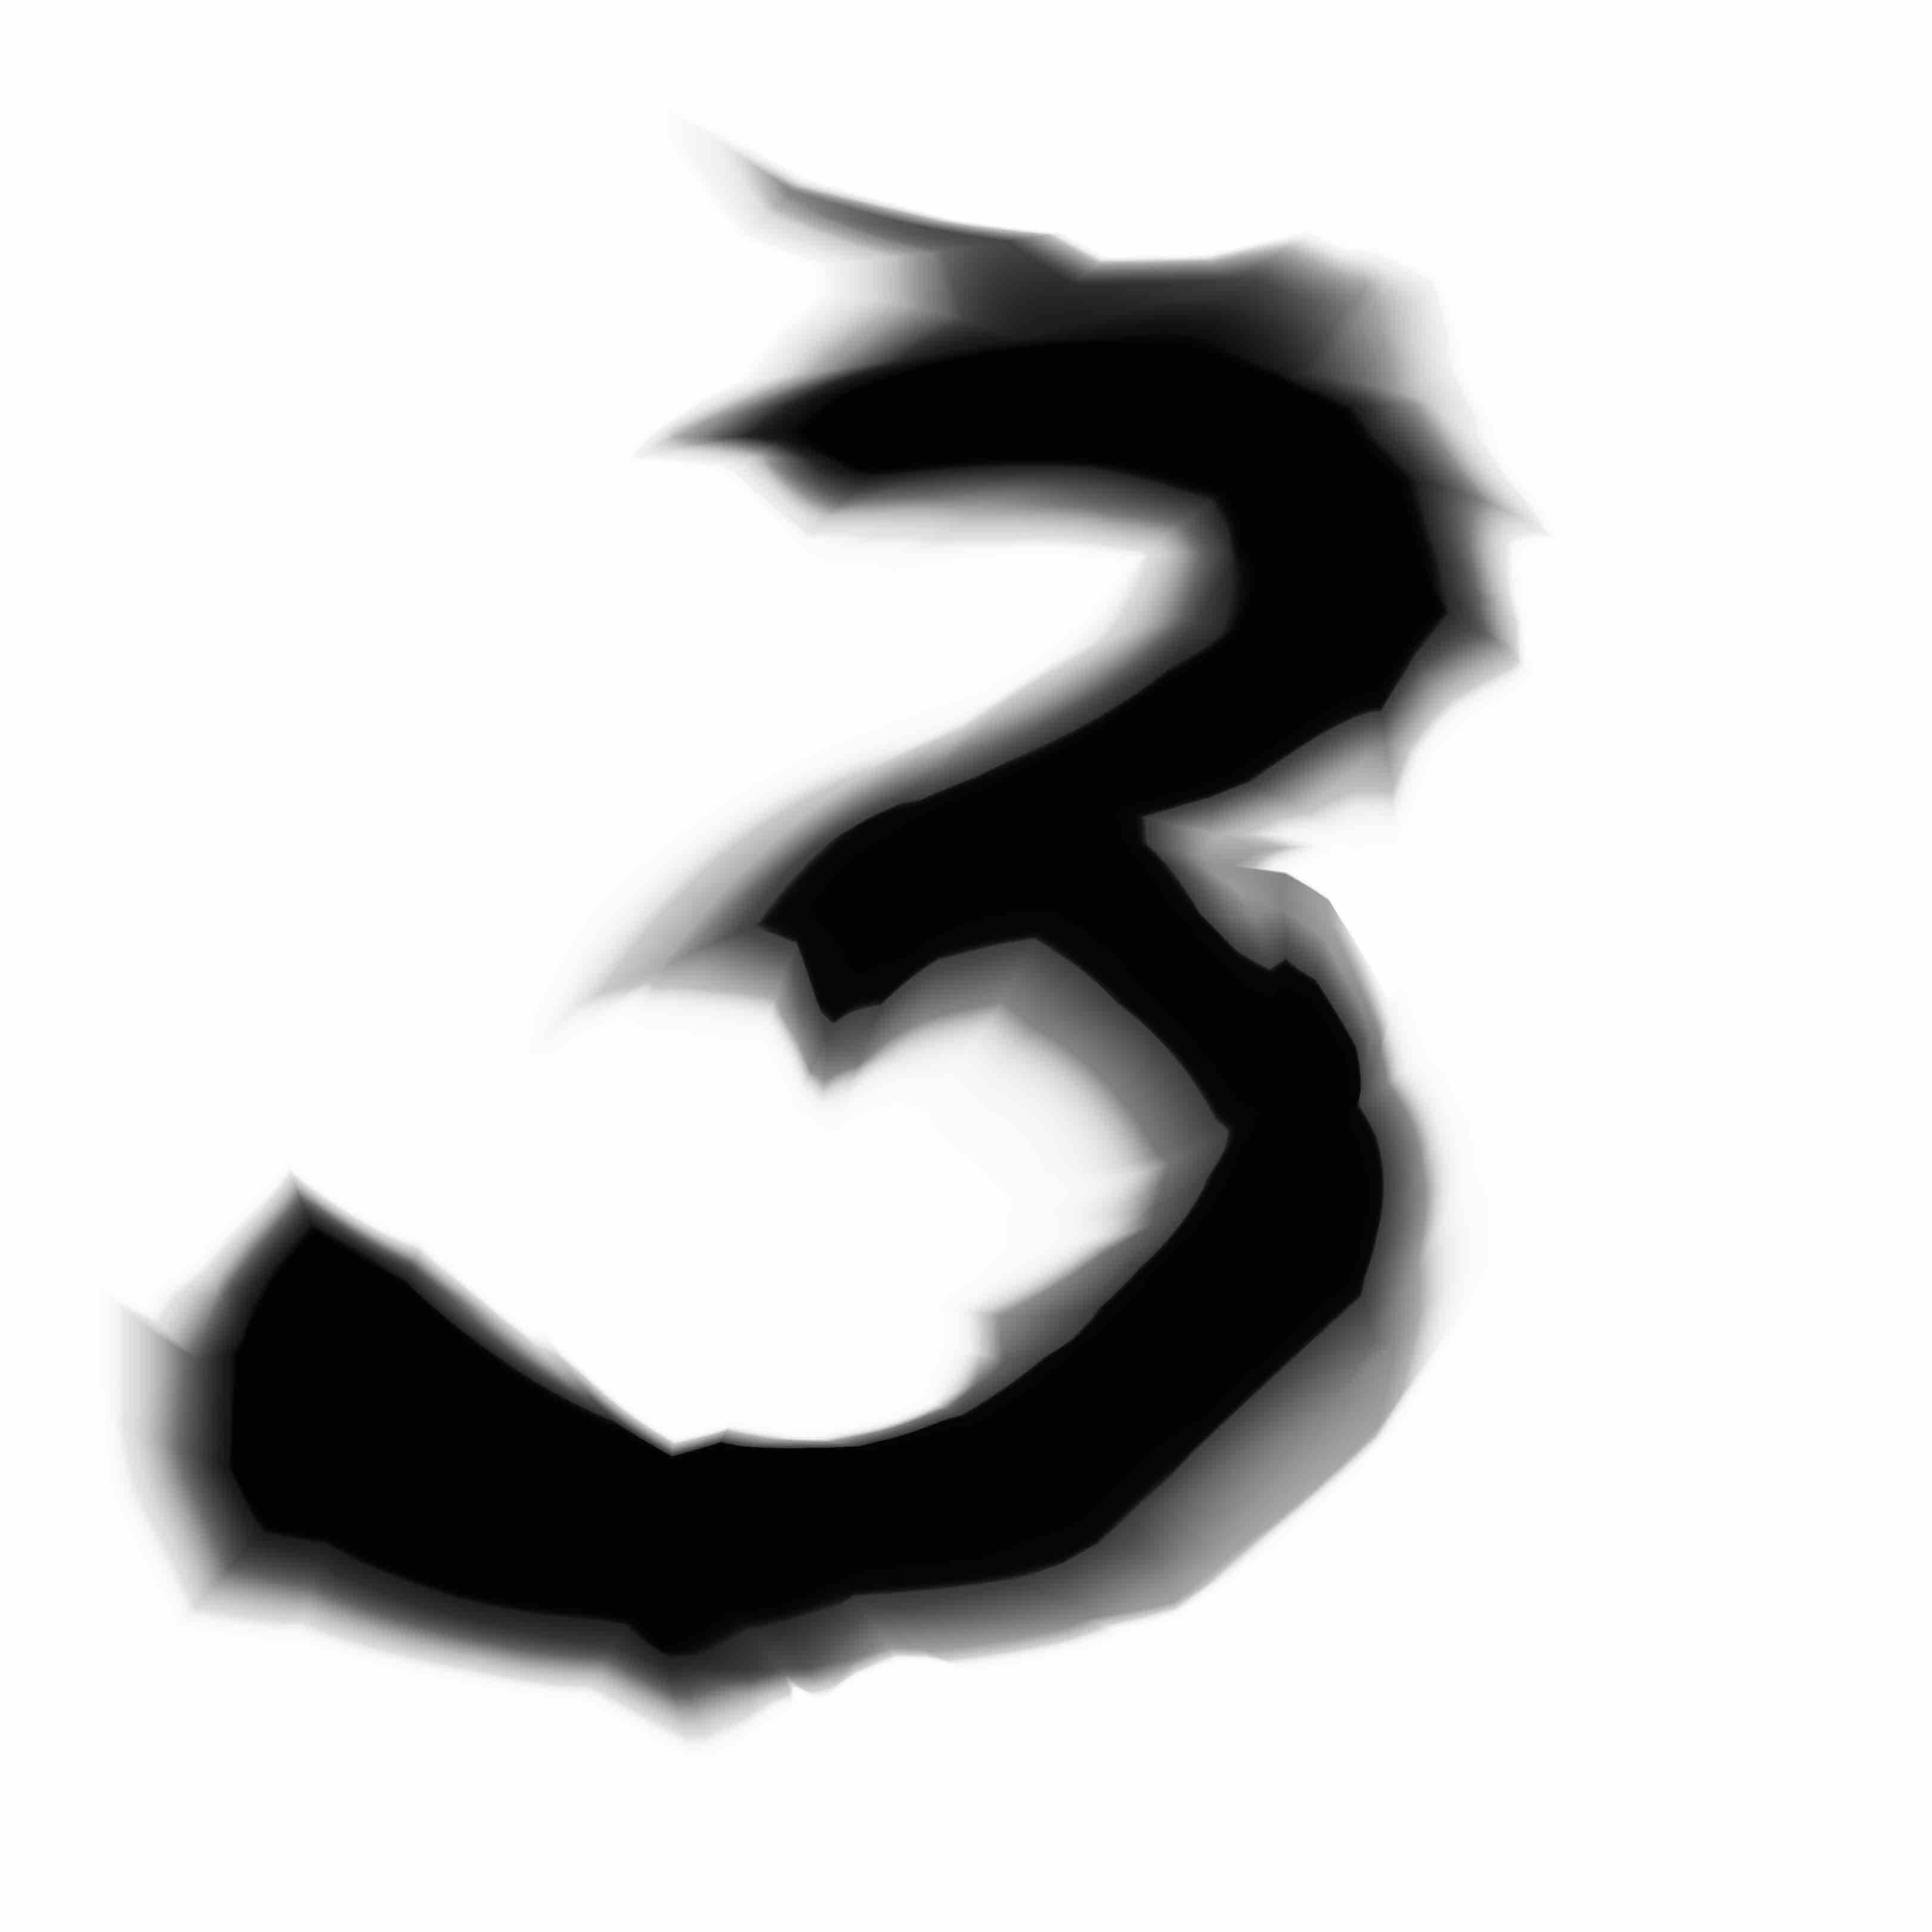
\includegraphics[width=.9\textwidth]{images/three.jpeg}};
\draw[black, thick] (9.7,3.5) rectangle (10.7,4.5);
\node[] at (10.2,3.2) {28*28};

\draw[->] (10.5,6.5) -- (neuron14);
\draw[->] (9.5,6.5) -- (neuron13);
\draw[->] (8.5,6.5) -- (neuron12);
\draw[->] (7.5,6.5) -- (neuron11);
\draw[->] (12.5,6.5) -- (neuron15);

\draw[red!20,dashed,line width=2pt] (neuron04) -- (neuron06);
\draw[green!20,dashed,line width=2pt] (neuron14) -- (neuron15);

\end{tikzpicture}
\end{center}
             
\tikzstyle{input_neuron}=[circle,draw=red!50,fill=red!10,thick,minimum size=6mm]
\tikzstyle{hidden_neuron}=[circle,draw=blue!50,fill=cyan!10,thick,minimum size=6mm]
\tikzstyle{output_neuron}=[circle,draw=green!50,fill=green!10,thick,minimum size=6mm]
\tikzstyle{cpy_neuron}=[circle,draw=green!50,fill=green!50,thick,minimum size=6mm]
\tikzstyle{input}=[circle,draw=black!50,fill=black!20,thick,minimum size=6mm]

\begin{center}
\begin{tikzpicture}

%\node [input_neuron] (neuron00) at (6.5,6) {} ;
\node [input_neuron] (neuron01) at (7.5,6) {} ;
\node [input_neuron] (neuron02) at (8.5,6)  {};
\node [input_neuron] (neuron03) at (9.5,6)  {};
\node [input_neuron] (neuron04) at (10.5,6)  {};
%\node [input_neuron] (neuron05) at (11.5,6)  {};
\node [input_neuron] (neuron06) at (12.5,6)  {};
%\node [input_neuron] (neuron07) at (13.5,6) {} ;

\node [output_neuron] (neuron11) at (7.5,7.5)  {$0$};
\node [output_neuron] (neuron12) at (8.5,7.5)  {$1$};
\node [output_neuron] (neuron13) at (9.5,7.5)  {$2$};
\node [cpy_neuron] (neuron14) at (10.5,7.5)  {$3$};
\node [output_neuron] (neuron15) at (12.5,7.5)  {$9$};


%\node[text width=0.01cm] at (12.2,4.5) {$x$};
%\node[text width=0.01cm] at (13.2,6) {$h$};
%\node[text width=0.01cm] at (12.2,7.5) {$\hat{x}$};

\draw[red!100,thick,solid,rounded corners=15pt] (7,5.5) rectangle (13,6.5);
%\draw[red!100,thick,solid,rounded corners=15pt] (8,7) rectangle (12,8);

\node[] at (10.2,5) {$|\textbf{x}_i| = 784 = 28 \times 28$};

\node[text width=0.5cm] at (10.2,4) 
 {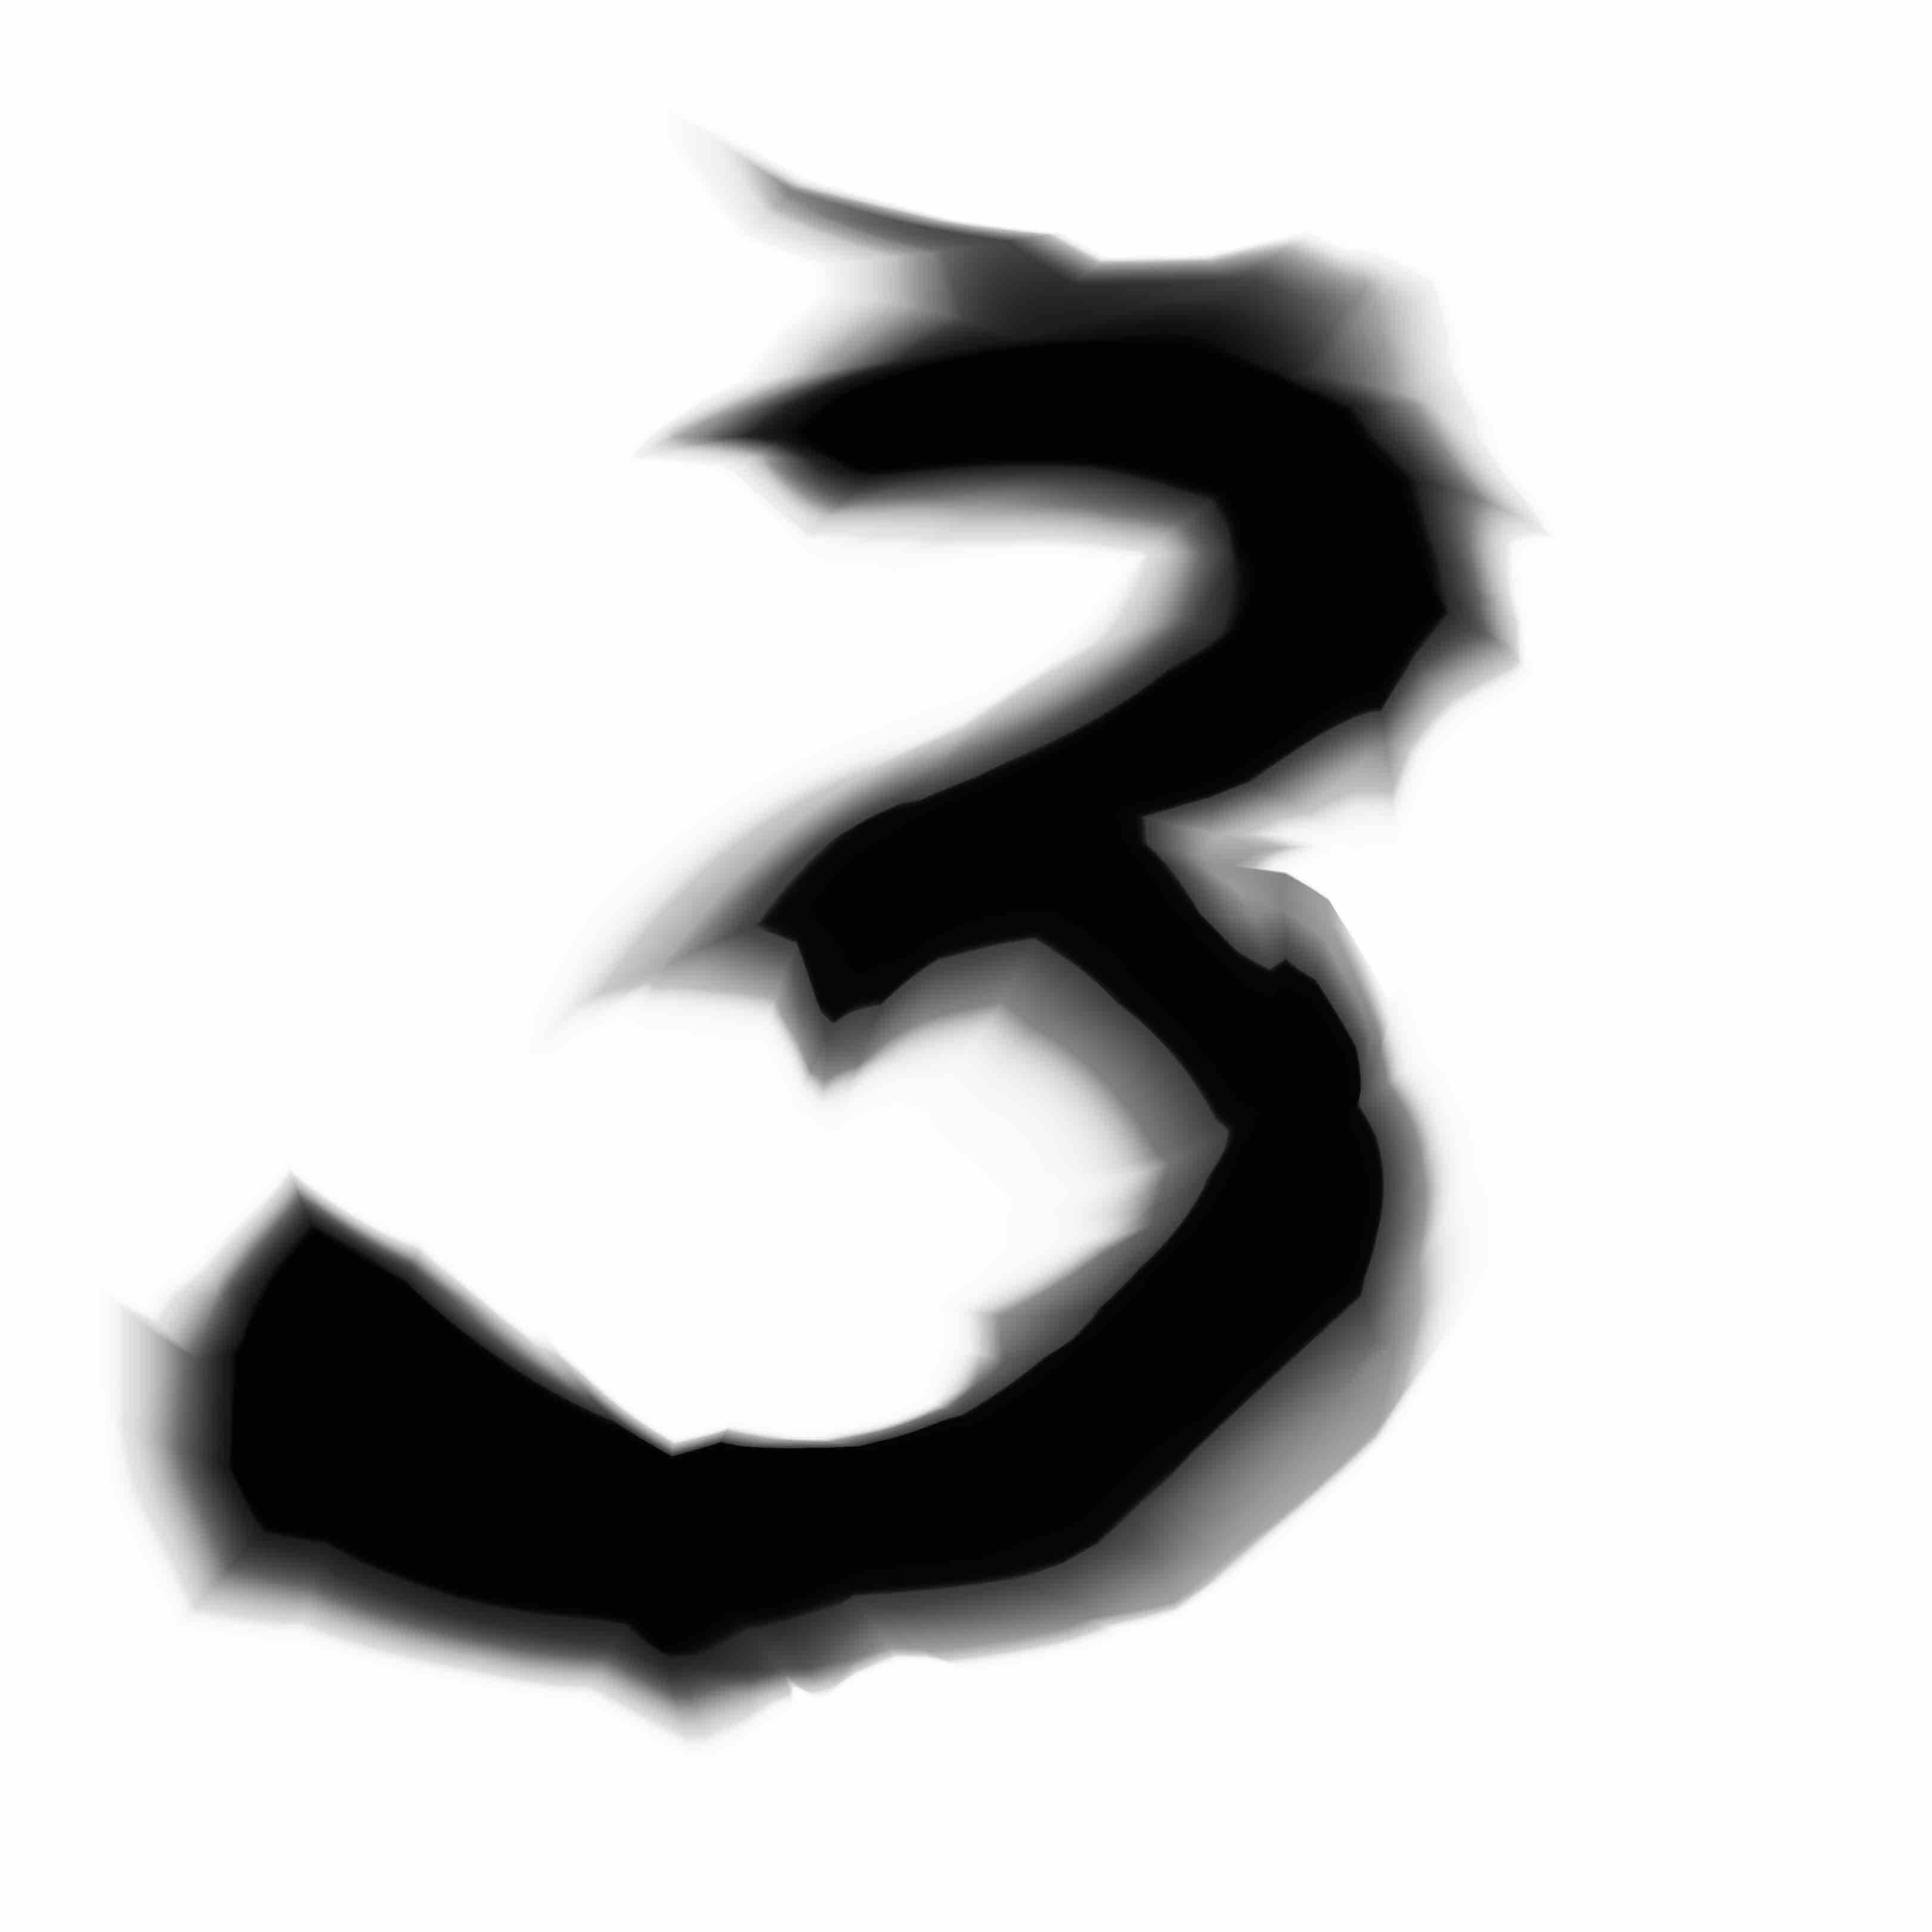
\includegraphics[width=.9\textwidth]{images/three.jpeg}};
\draw[black, thick] (9.7,3.5) rectangle (10.7,4.5);
\node[] at (10.2,3.2) {28*28};

\draw[->] (10.5,6.5) -- (neuron14);
\draw[->] (9.5,6.5) -- (neuron13);
\draw[->] (8.5,6.5) -- (neuron12);
\draw[->] (7.5,6.5) -- (neuron11);
\draw[->] (12.5,6.5) -- (neuron15);

\draw[red!20,dashed,line width=2pt] (neuron04) -- (neuron06);
\draw[green!20,dashed,line width=2pt] (neuron14) -- (neuron15);

\end{tikzpicture}
\end{center}
            \caption{Basic approach(we use raw data as input features)}
        \end{figure}

    \end{overlayarea}

  \end{columns}
\end{frame}

\begin{frame}
  \begin{columns}
    \column{0.4\textwidth}

    \begin{overlayarea}{\textwidth}{\textheight}
        \vspace{0.2in}
        \textbf{\large{Task: Hand-written digit recognition}}
        \begin{figure}
            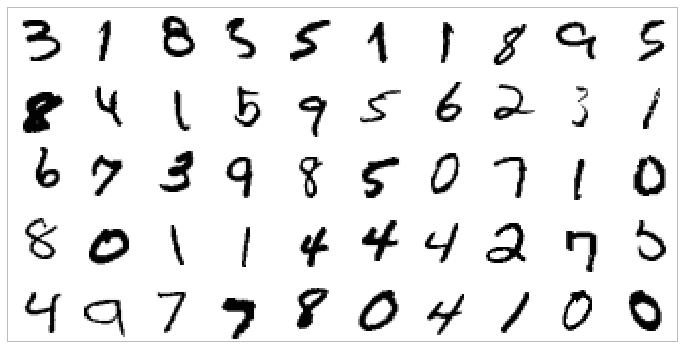
\includegraphics[scale= 0.25]{images/mnist.png}
        \caption{MNIST Data}
        \end{figure}
    \end{overlayarea}

    \column{0.6\textwidth}
    \begin{overlayarea}{\textwidth}{\textheight}
    \begin{figure}
            \hspace{2cm}
			
\begin{tikzpicture}
	\tikzstyle{input_neuron}=[circle,draw=red!50,fill=red!10,thick,minimum size=6mm]
	\tikzstyle{hidden_neuron}=[circle,draw=blue!50,fill=cyan!10,thick,minimum size=6mm]
	\tikzstyle{output_neuron}=[circle,draw=green!50,fill=green!10,thick,minimum size=6mm]
	\tikzstyle{cpy_neuron}=[circle,draw=red!50,fill=red!50,thick,minimum size=6mm]
	\tikzstyle{input}=[circle,draw=black!50,fill=black!20,thick,minimum size=6mm]

	\node [input_neuron] (neuron00) at (7.5,4.5) {};
	\node [input_neuron] (neuron01) at (8.5,4.5) {};
	\node [input_neuron] (neuron02) at (9.5,4.5){};
	\node [input_neuron] (neuron03) at (10.5,4.5) {};
	%\node [input_neuron] (neuron04) at (11.5,4.5) {};
	\node [input_neuron] (neuron05) at (12.5,4.5) {};

	%\node [hidden_neuron] (neuron51) at (7.5,6) {} ;
	\node [hidden_neuron] (neuron52) at (8.5,6)  {};
	\node [hidden_neuron] (neuron53) at (9.5,6)  {};
	%\node [hidden_neuron] (neuron54) at (10.5,6)  {};
	\node [hidden_neuron] (neuron55) at (11.5,6)  {};
	%\node [hidden_neuron] (neuron56) at (12.5,6)  {};

	\node [output_neuron] (neuron10) at (7.5,7.5)  {};
	\node [output_neuron] (neuron11) at (8.5,7.5)  {};
	\node [output_neuron] (neuron12) at (9.5,7.5)  {};
	\node [output_neuron] (neuron13) at (10.5,7.5)  {};
	%\node [output_neuron] (neuron14) at (11.5,7.5)  {};
	\node [output_neuron] (neuron14) at (12.5,7.5)  {};

	\draw[red!100,thick,solid,rounded corners=15pt] (7,4) rectangle (13,5);
	\draw[red!100,thick,solid,rounded corners=15pt] (8,5.5) rectangle (12,6.5);
	\draw[red!100,thick,solid,rounded corners=15pt] (7,7) rectangle (13,8);

	%\draw[black!50,thick,solid] (7,5) -- (8,5.5);
	%\draw[black!50,thick,solid] (13,5) -- (12,5.5);
	%\draw[black!50,thick,solid] (8,6.5) -- (7,7);
	%\draw[black!50,thick,solid] (12,6.5) -- (13,7);        
	\draw[thick,->] (10,5) -- (10,5.5);

	\draw[thick,->] (10,6.5) -- (10,7);

	%\node[] at (7.4,6) {\textbf{•}xtbf{h}};     

	\draw[red!20,dashed,line width=2pt] (neuron03) -- (neuron05);
	\draw[blue!20,dashed,line width=2pt] (neuron53) -- (neuron55);
	\draw[green!20,dashed,line width=2pt] (neuron13) -- (neuron14);        

	\node[] at (10,3.5) {$|\textbf{x}_i| = 784 = 28 \times 28$};
	\node[] at (13.9,8) {$\hat{\textbf{x}}_i \in \mathbb{R}^{784}$};
	\node[] at (13,6) {$\textbf{h} \in \mathbb{R}^{d}$};      
	\node[text width=0.5cm] at (10,2.5) 
	    {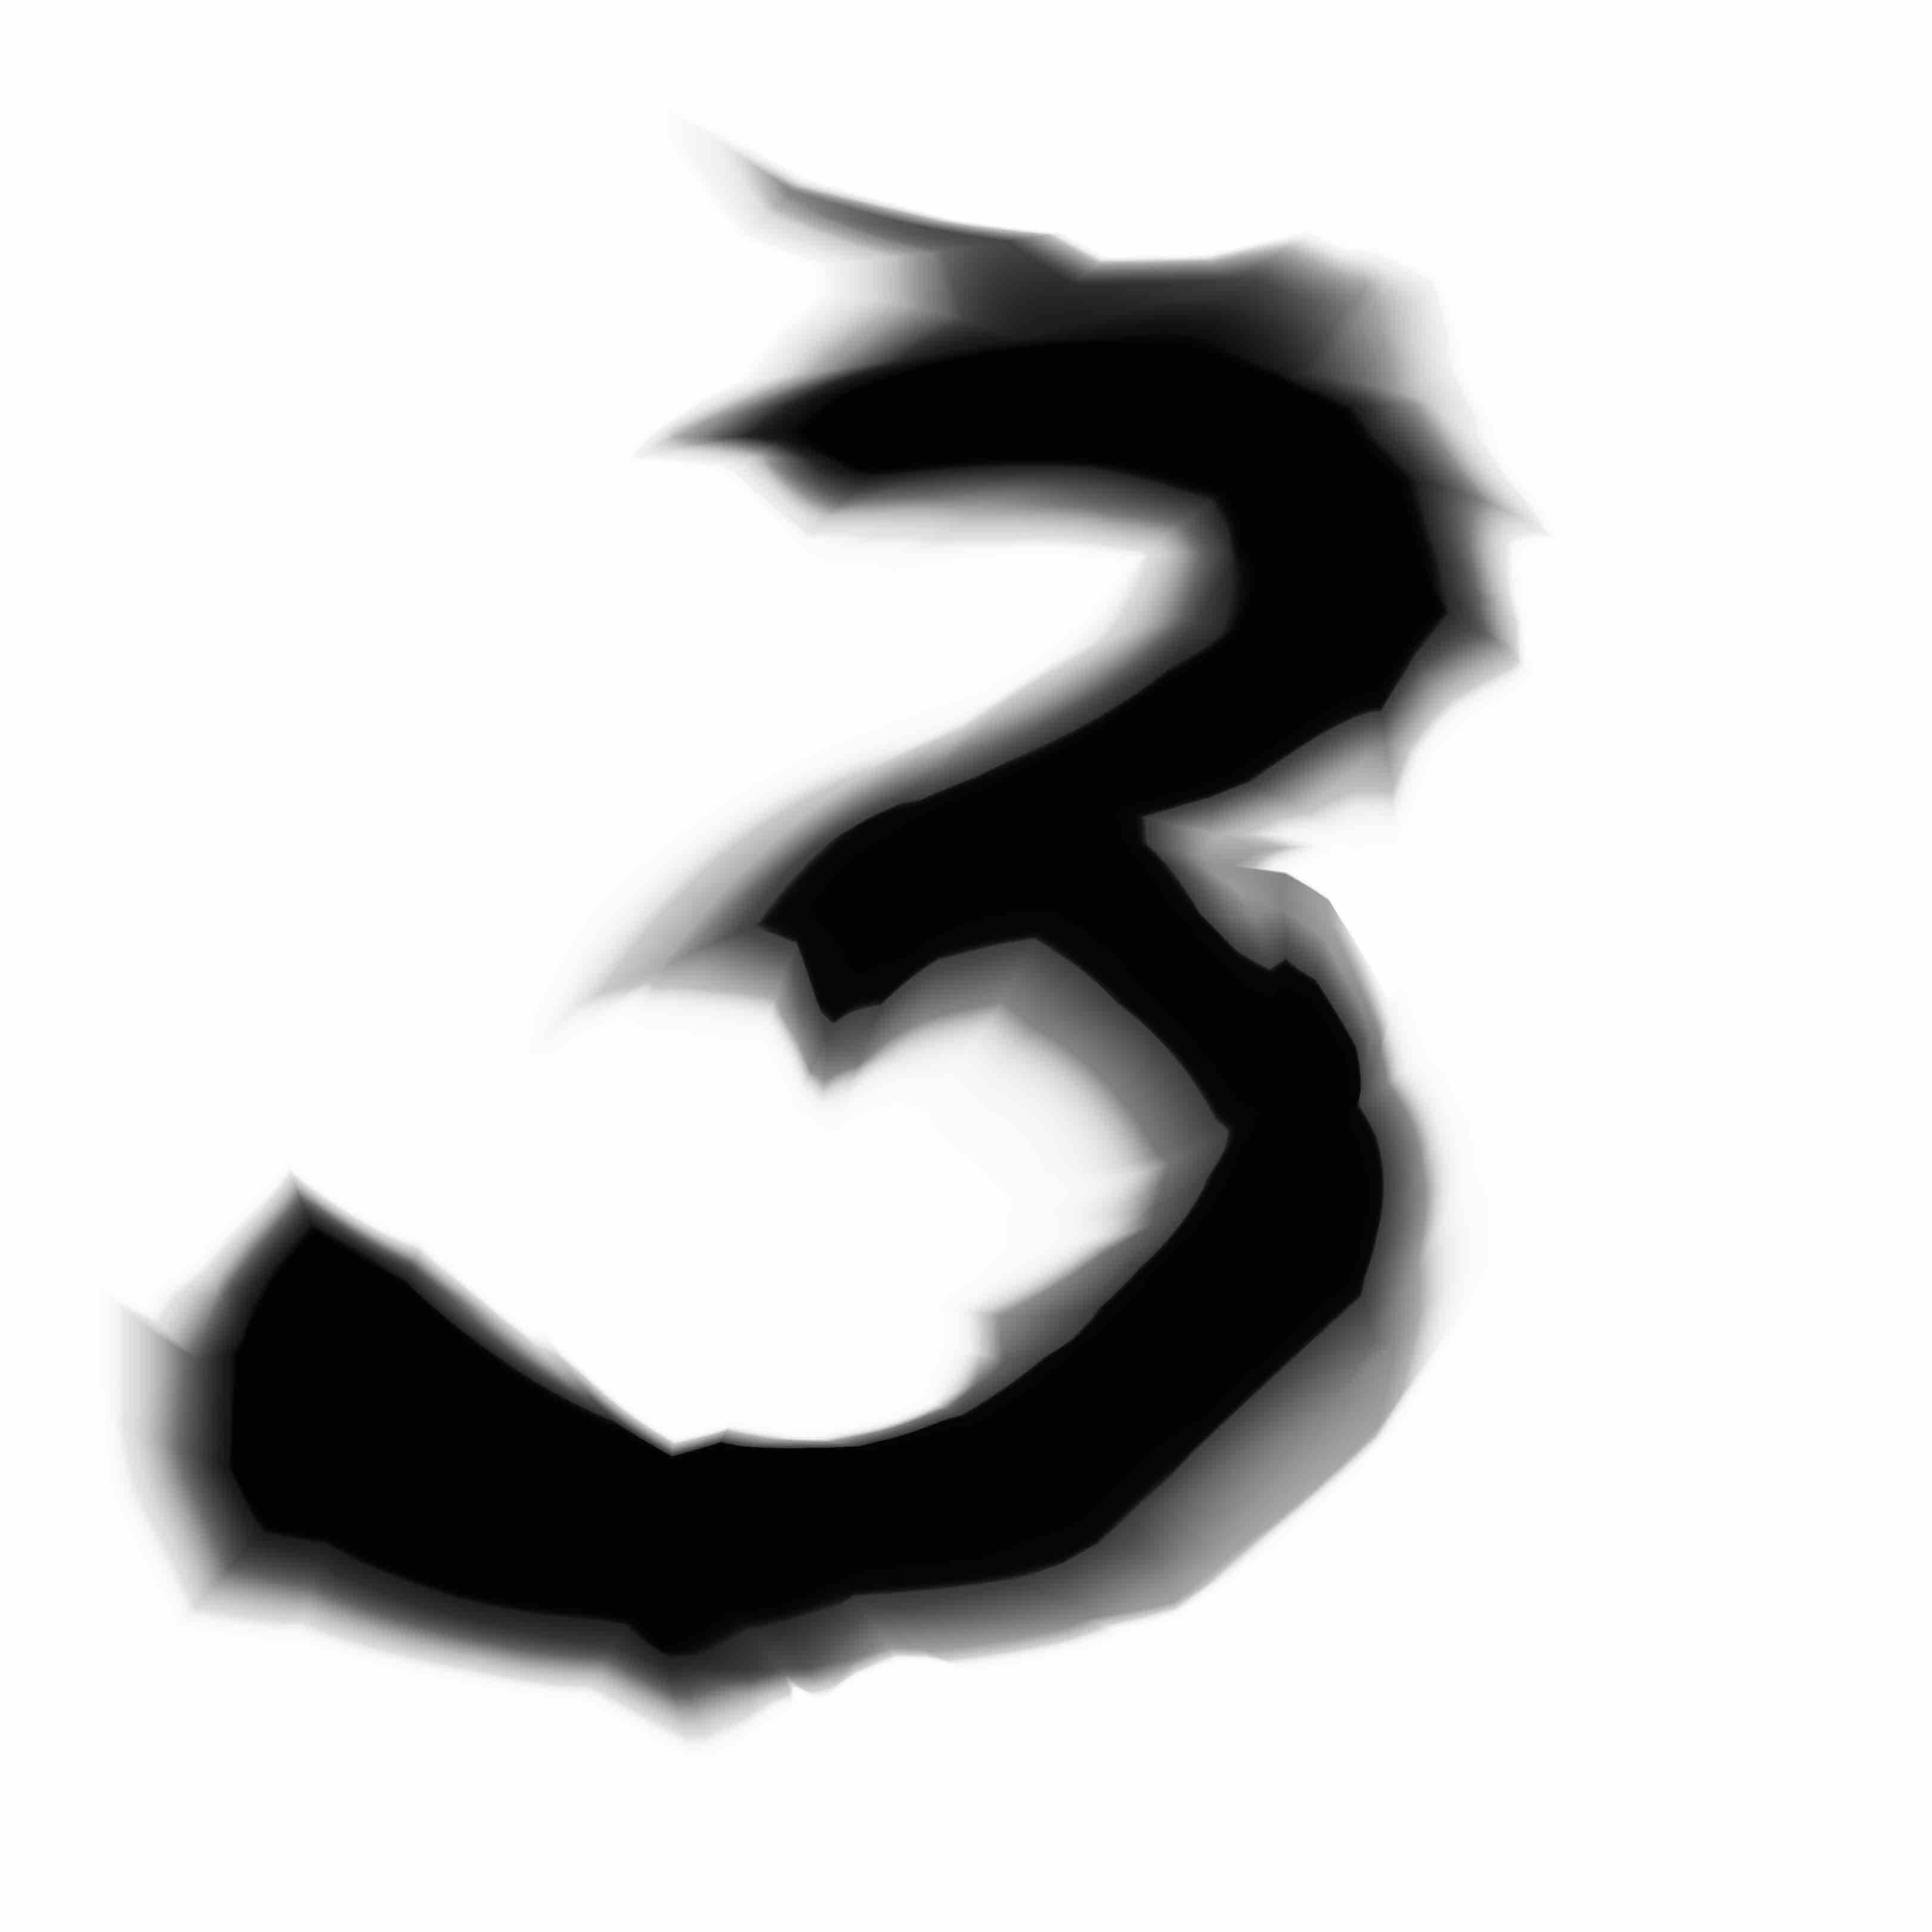
\includegraphics[width=.9\textwidth]{images/three.jpeg}};
	\draw[black, thick] (9.5,2) rectangle (10.5,3);             
        
\end{tikzpicture}

            \vspace{0.3cm}
        \caption{\small{AE approach (first learn important characteristics of data)}} 
    \end{figure}
 
    \end{overlayarea}
  \end{columns}
\end{frame}

\begin{frame}
  \begin{columns}
    \column{0.4\textwidth}

    \begin{overlayarea}{\textwidth}{\textheight}
        \vspace{0.2in}
        \textbf{\large{Task: Hand-written digit recognition}}
        \begin{figure}
            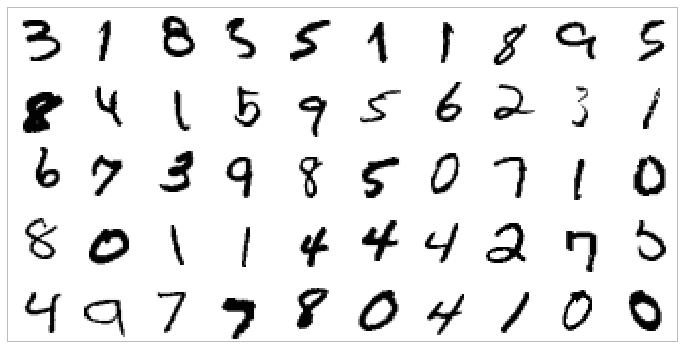
\includegraphics[scale= 0.25]{images/mnist.png}
        \caption{MNIST Data}
        \end{figure}
    \end{overlayarea}

      \column{0.6\textwidth}
      
    \begin{overlayarea}{\textwidth}{\textheight}

            \begin{figure}
        \hspace{2cm}
        %         \tikzstyle{input_neuron}=[circle,draw=red!50,fill=red!10,thick,minimum size=6mm]
		\tikzstyle{hidden_neuron}=[circle,draw=blue!50,fill=cyan!10,thick,minimum size=6mm]
		\tikzstyle{output_neuron}=[circle,draw=green!50,fill=green!10,thick,minimum size=6mm]
		\tikzstyle{cpy_neuron}=[circle,draw=red!50,fill=red!50,thick,minimum size=6mm]
		\tikzstyle{input}=[circle,draw=black!50,fill=black!20,thick,minimum size=6mm]

\begin{center}

\begin{tikzpicture}

		\node [input_neuron] (neuron00) at (7.5,4.5) {};
        \node [input_neuron] (neuron01) at (8.5,4.5) {};
		\node [input_neuron] (neuron02) at (9.5,4.5){};
		\node [input_neuron] (neuron03) at (10.5,4.5) {};
		%\node [input_neuron] (neuron04) at (11.5,4.5) {};
		\node [input_neuron] (neuron05) at (12.5,4.5) {};
		
		%\node [hidden_neuron] (neuron51) at (7.5,6) {} ;
		\node [hidden_neuron] (neuron52) at (8.5,6)  {};
		\node [hidden_neuron] (neuron53) at (9.5,6)  {};
		%\node [hidden_neuron] (neuron54) at (10.5,6)  {};
		\node [hidden_neuron] (neuron55) at (11.5,6)  {};
		%\node [hidden_neuron] (neuron56) at (12.5,6)  {};
		
		\node [output_neuron] (neuron10) at (7.5,7.5)  {$0$};
		\node [output_neuron] (neuron11) at (8.5,7.5)  {$1$};
		\node [output_neuron] (neuron12) at (9.5,7.5)  {$2$};
		\node [output_neuron] (neuron13) at (10.5,7.5)  {$3$};
		%\node [output_neuron] (neuron14) at (11.5,7.5)  {};
		\node [output_neuron] (neuron14) at (12.5,7.5)  {$9$};
		
		\draw[red!100,thick,solid,rounded corners=15pt] (7,4) rectangle (13,5);
		\draw[red!100,thick,solid,rounded corners=15pt] (8,5.5) rectangle (12,6.5);
		%\draw[red!100,thick,solid,rounded corners=15pt] (7,7) rectangle (13,8);
		
		%\draw[black!50,thick,solid] (7,5) -- (8,5.5);
		%\draw[black!50,thick,solid] (13,5) -- (12,5.5);
		%\draw[black!50,thick,solid] (8,6.5) -- (7,7);
		%\draw[black!50,thick,solid] (12,6.5) -- (13,7);		
		%\draw[thick,->] (10,5) -- (10,5.5);
		%\draw[thick,->] (10,6.5) -- (10,7);
		
		\foreach \x in {neuron10,neuron11,neuron12,neuron13,neuron14}
			\draw[thick,->] (10,6.5) -- (\x);
		
		%\node[] at (7.4,6) {\textbf{h}};		
		
		\draw[thick,->] (10,5) -- (10,5.5);
		
		
		\draw[red!20,dashed,line width=2pt] (neuron03) -- (neuron05);
		\draw[blue!20,dashed,line width=2pt] (neuron53) -- (neuron55);
		\draw[green!20,dashed,line width=2pt] (neuron13) -- (neuron14);        
		
		\node[] at (10,3.5) {$|\textbf{x}_i| = 784 = 28 \times 28$};
		%\node[] at (13.5,8) {$\hat{x} \in \mathbb{R}^{784}$};
		\node[] at (13,6) {$\textbf{h} \in \mathbb{R}^{d}$};		
		\node[text width=0.5cm] at (10,2.5) 
 			{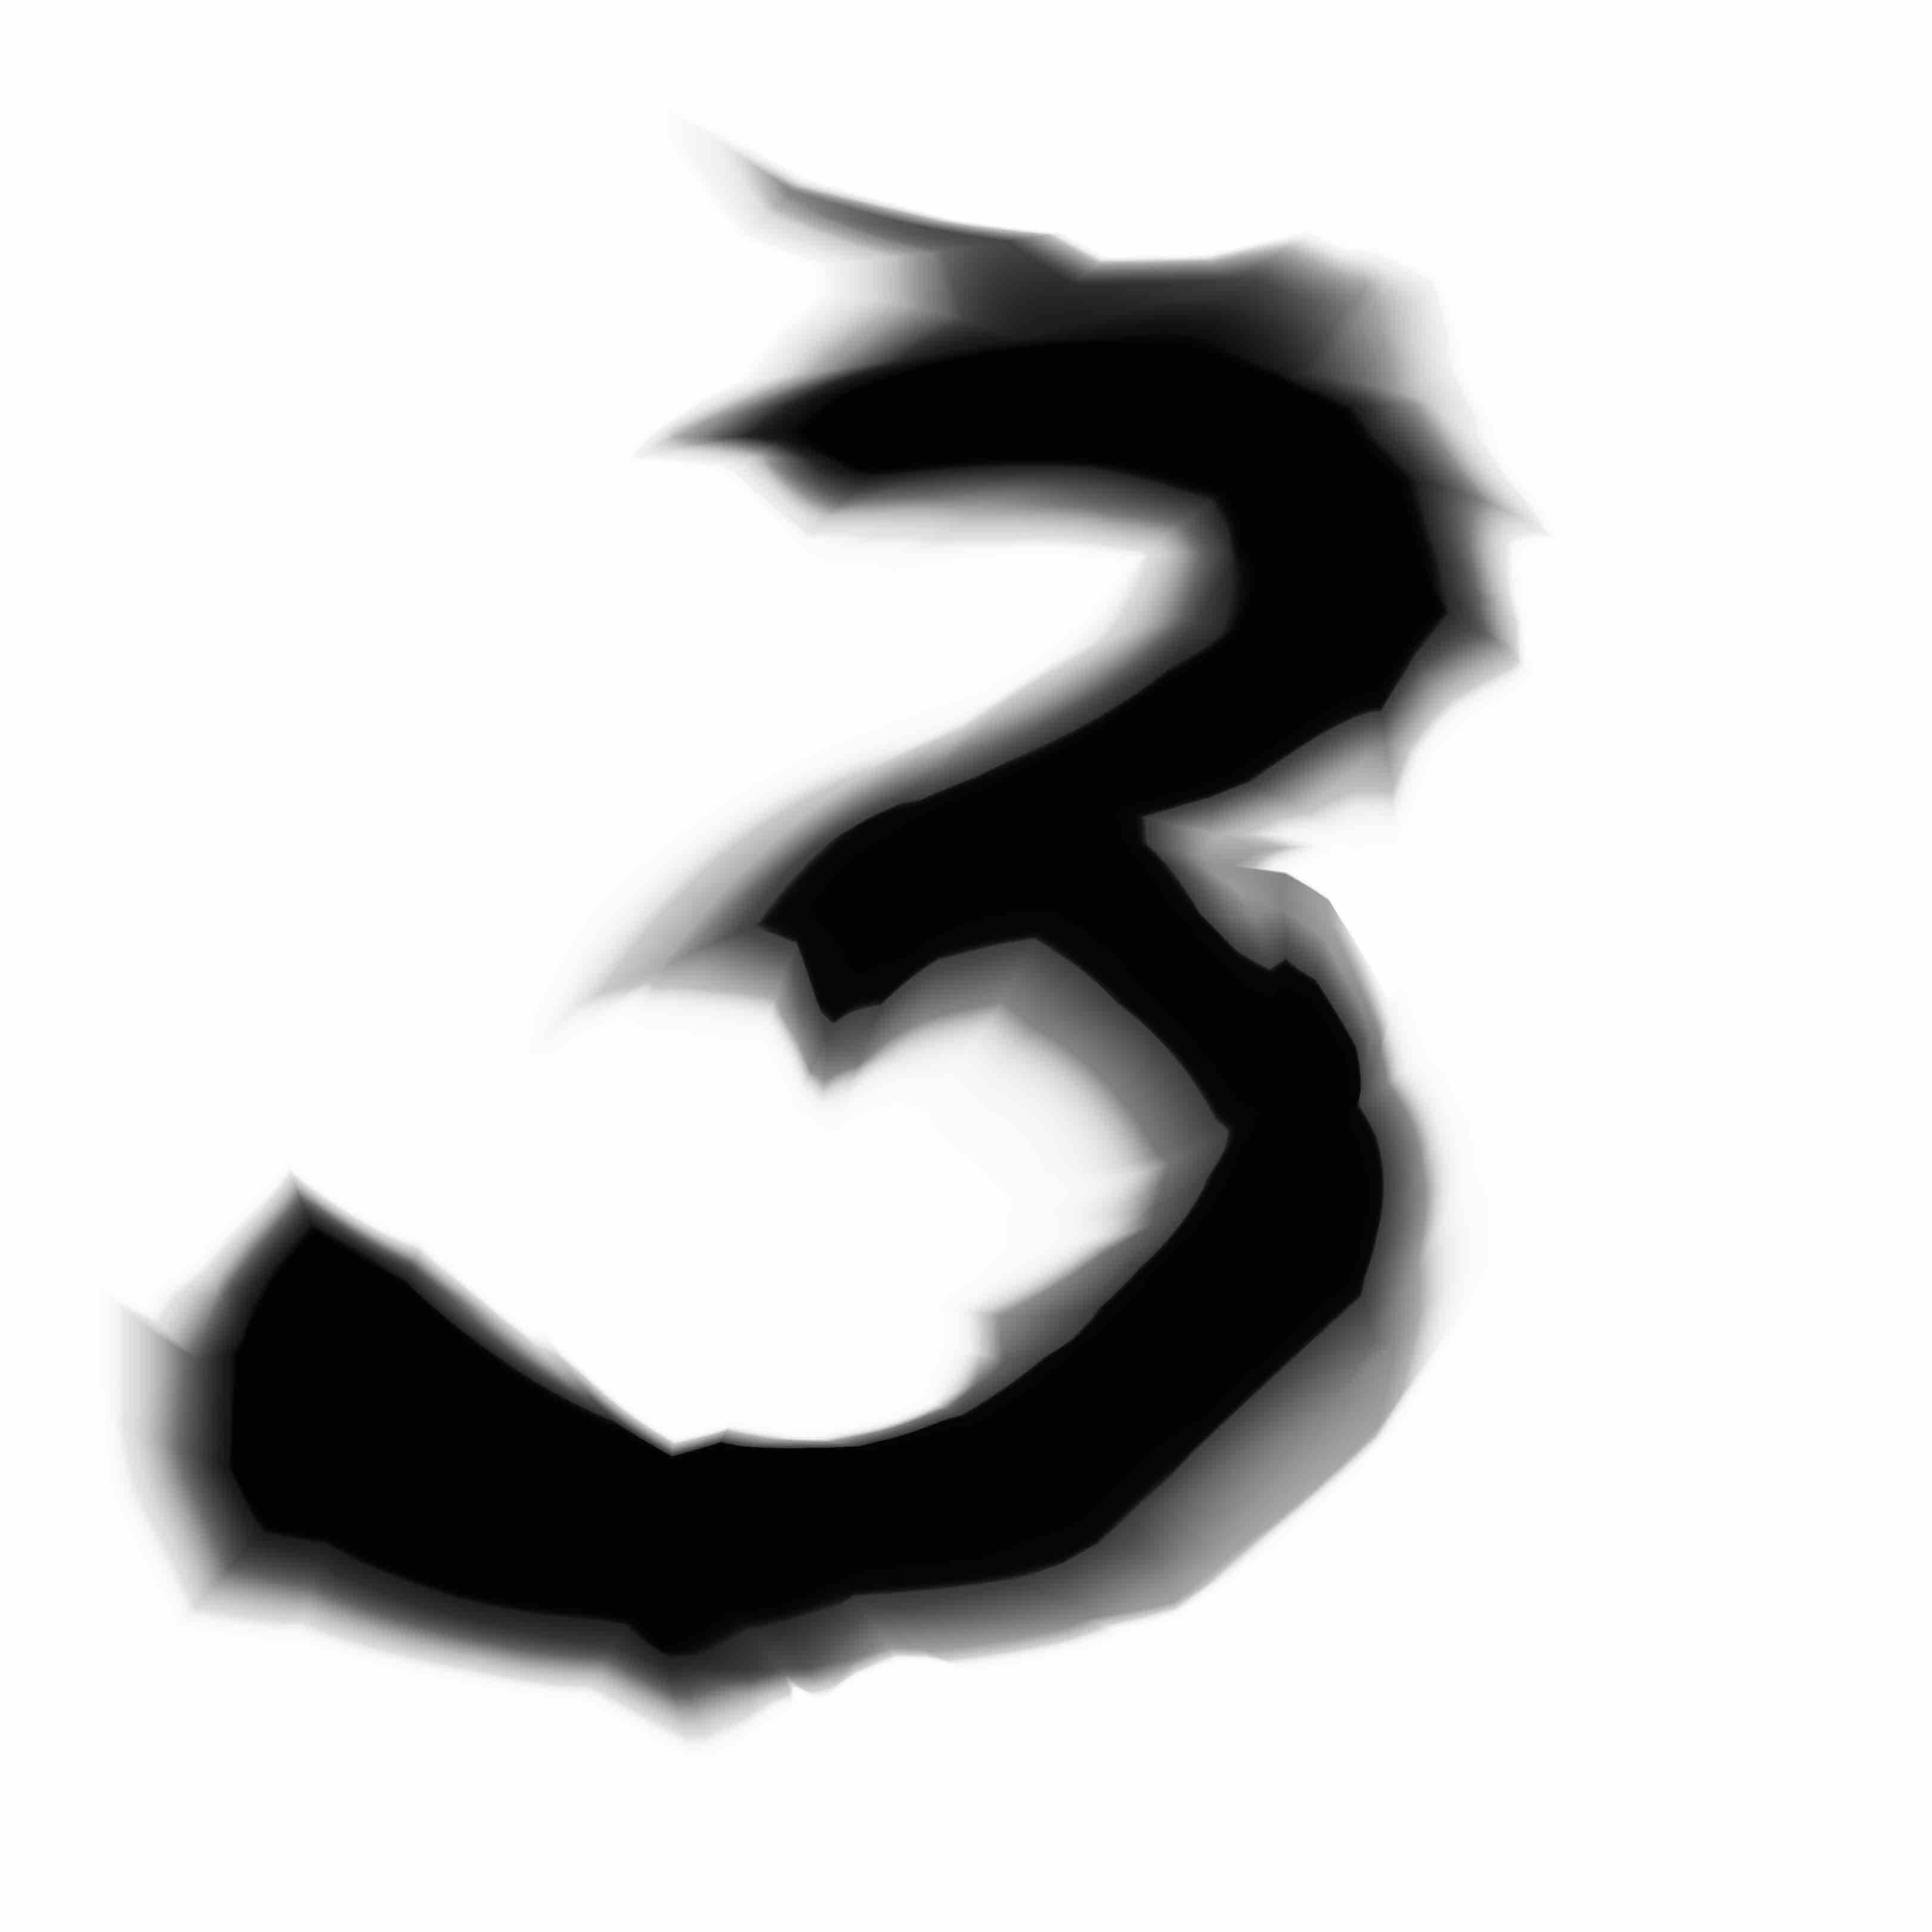
\includegraphics[width=.9\textwidth]{images/three.jpeg}};
		\draw[black, thick] (9.5,2) rectangle (10.5,3);				
		
\end{tikzpicture}

\end{center}
                \tikzstyle{input_neuron}=[circle,draw=red!50,fill=red!10,thick,minimum size=6mm]
		\tikzstyle{hidden_neuron}=[circle,draw=blue!50,fill=cyan!10,thick,minimum size=6mm]
		\tikzstyle{output_neuron}=[circle,draw=green!50,fill=green!10,thick,minimum size=6mm]
		\tikzstyle{cpy_neuron}=[circle,draw=red!50,fill=red!50,thick,minimum size=6mm]
		\tikzstyle{input}=[circle,draw=black!50,fill=black!20,thick,minimum size=6mm]

\begin{center}

\begin{tikzpicture}

		\node [input_neuron] (neuron00) at (7.5,4.5) {};
        \node [input_neuron] (neuron01) at (8.5,4.5) {};
		\node [input_neuron] (neuron02) at (9.5,4.5){};
		\node [input_neuron] (neuron03) at (10.5,4.5) {};
		%\node [input_neuron] (neuron04) at (11.5,4.5) {};
		\node [input_neuron] (neuron05) at (12.5,4.5) {};
		
		%\node [hidden_neuron] (neuron51) at (7.5,6) {} ;
		\node [hidden_neuron] (neuron52) at (8.5,6)  {};
		\node [hidden_neuron] (neuron53) at (9.5,6)  {};
		%\node [hidden_neuron] (neuron54) at (10.5,6)  {};
		\node [hidden_neuron] (neuron55) at (11.5,6)  {};
		%\node [hidden_neuron] (neuron56) at (12.5,6)  {};
		
		\node [output_neuron] (neuron10) at (7.5,7.5)  {$0$};
		\node [output_neuron] (neuron11) at (8.5,7.5)  {$1$};
		\node [output_neuron] (neuron12) at (9.5,7.5)  {$2$};
		\node [output_neuron] (neuron13) at (10.5,7.5)  {$3$};
		%\node [output_neuron] (neuron14) at (11.5,7.5)  {};
		\node [output_neuron] (neuron14) at (12.5,7.5)  {$9$};
		
		\draw[red!100,thick,solid,rounded corners=15pt] (7,4) rectangle (13,5);
		\draw[red!100,thick,solid,rounded corners=15pt] (8,5.5) rectangle (12,6.5);
		%\draw[red!100,thick,solid,rounded corners=15pt] (7,7) rectangle (13,8);
		
		%\draw[black!50,thick,solid] (7,5) -- (8,5.5);
		%\draw[black!50,thick,solid] (13,5) -- (12,5.5);
		%\draw[black!50,thick,solid] (8,6.5) -- (7,7);
		%\draw[black!50,thick,solid] (12,6.5) -- (13,7);		
		%\draw[thick,->] (10,5) -- (10,5.5);
		%\draw[thick,->] (10,6.5) -- (10,7);
		
		\foreach \x in {neuron10,neuron11,neuron12,neuron13,neuron14}
			\draw[thick,->] (10,6.5) -- (\x);
		
		%\node[] at (7.4,6) {\textbf{h}};		
		
		\draw[thick,->] (10,5) -- (10,5.5);
		
		
		\draw[red!20,dashed,line width=2pt] (neuron03) -- (neuron05);
		\draw[blue!20,dashed,line width=2pt] (neuron53) -- (neuron55);
		\draw[green!20,dashed,line width=2pt] (neuron13) -- (neuron14);        
		
		\node[] at (10,3.5) {$|\textbf{x}_i| = 784 = 28 \times 28$};
		%\node[] at (13.5,8) {$\hat{x} \in \mathbb{R}^{784}$};
		\node[] at (13,6) {$\textbf{h} \in \mathbb{R}^{d}$};		
		\node[text width=0.5cm] at (10,2.5) 
 			{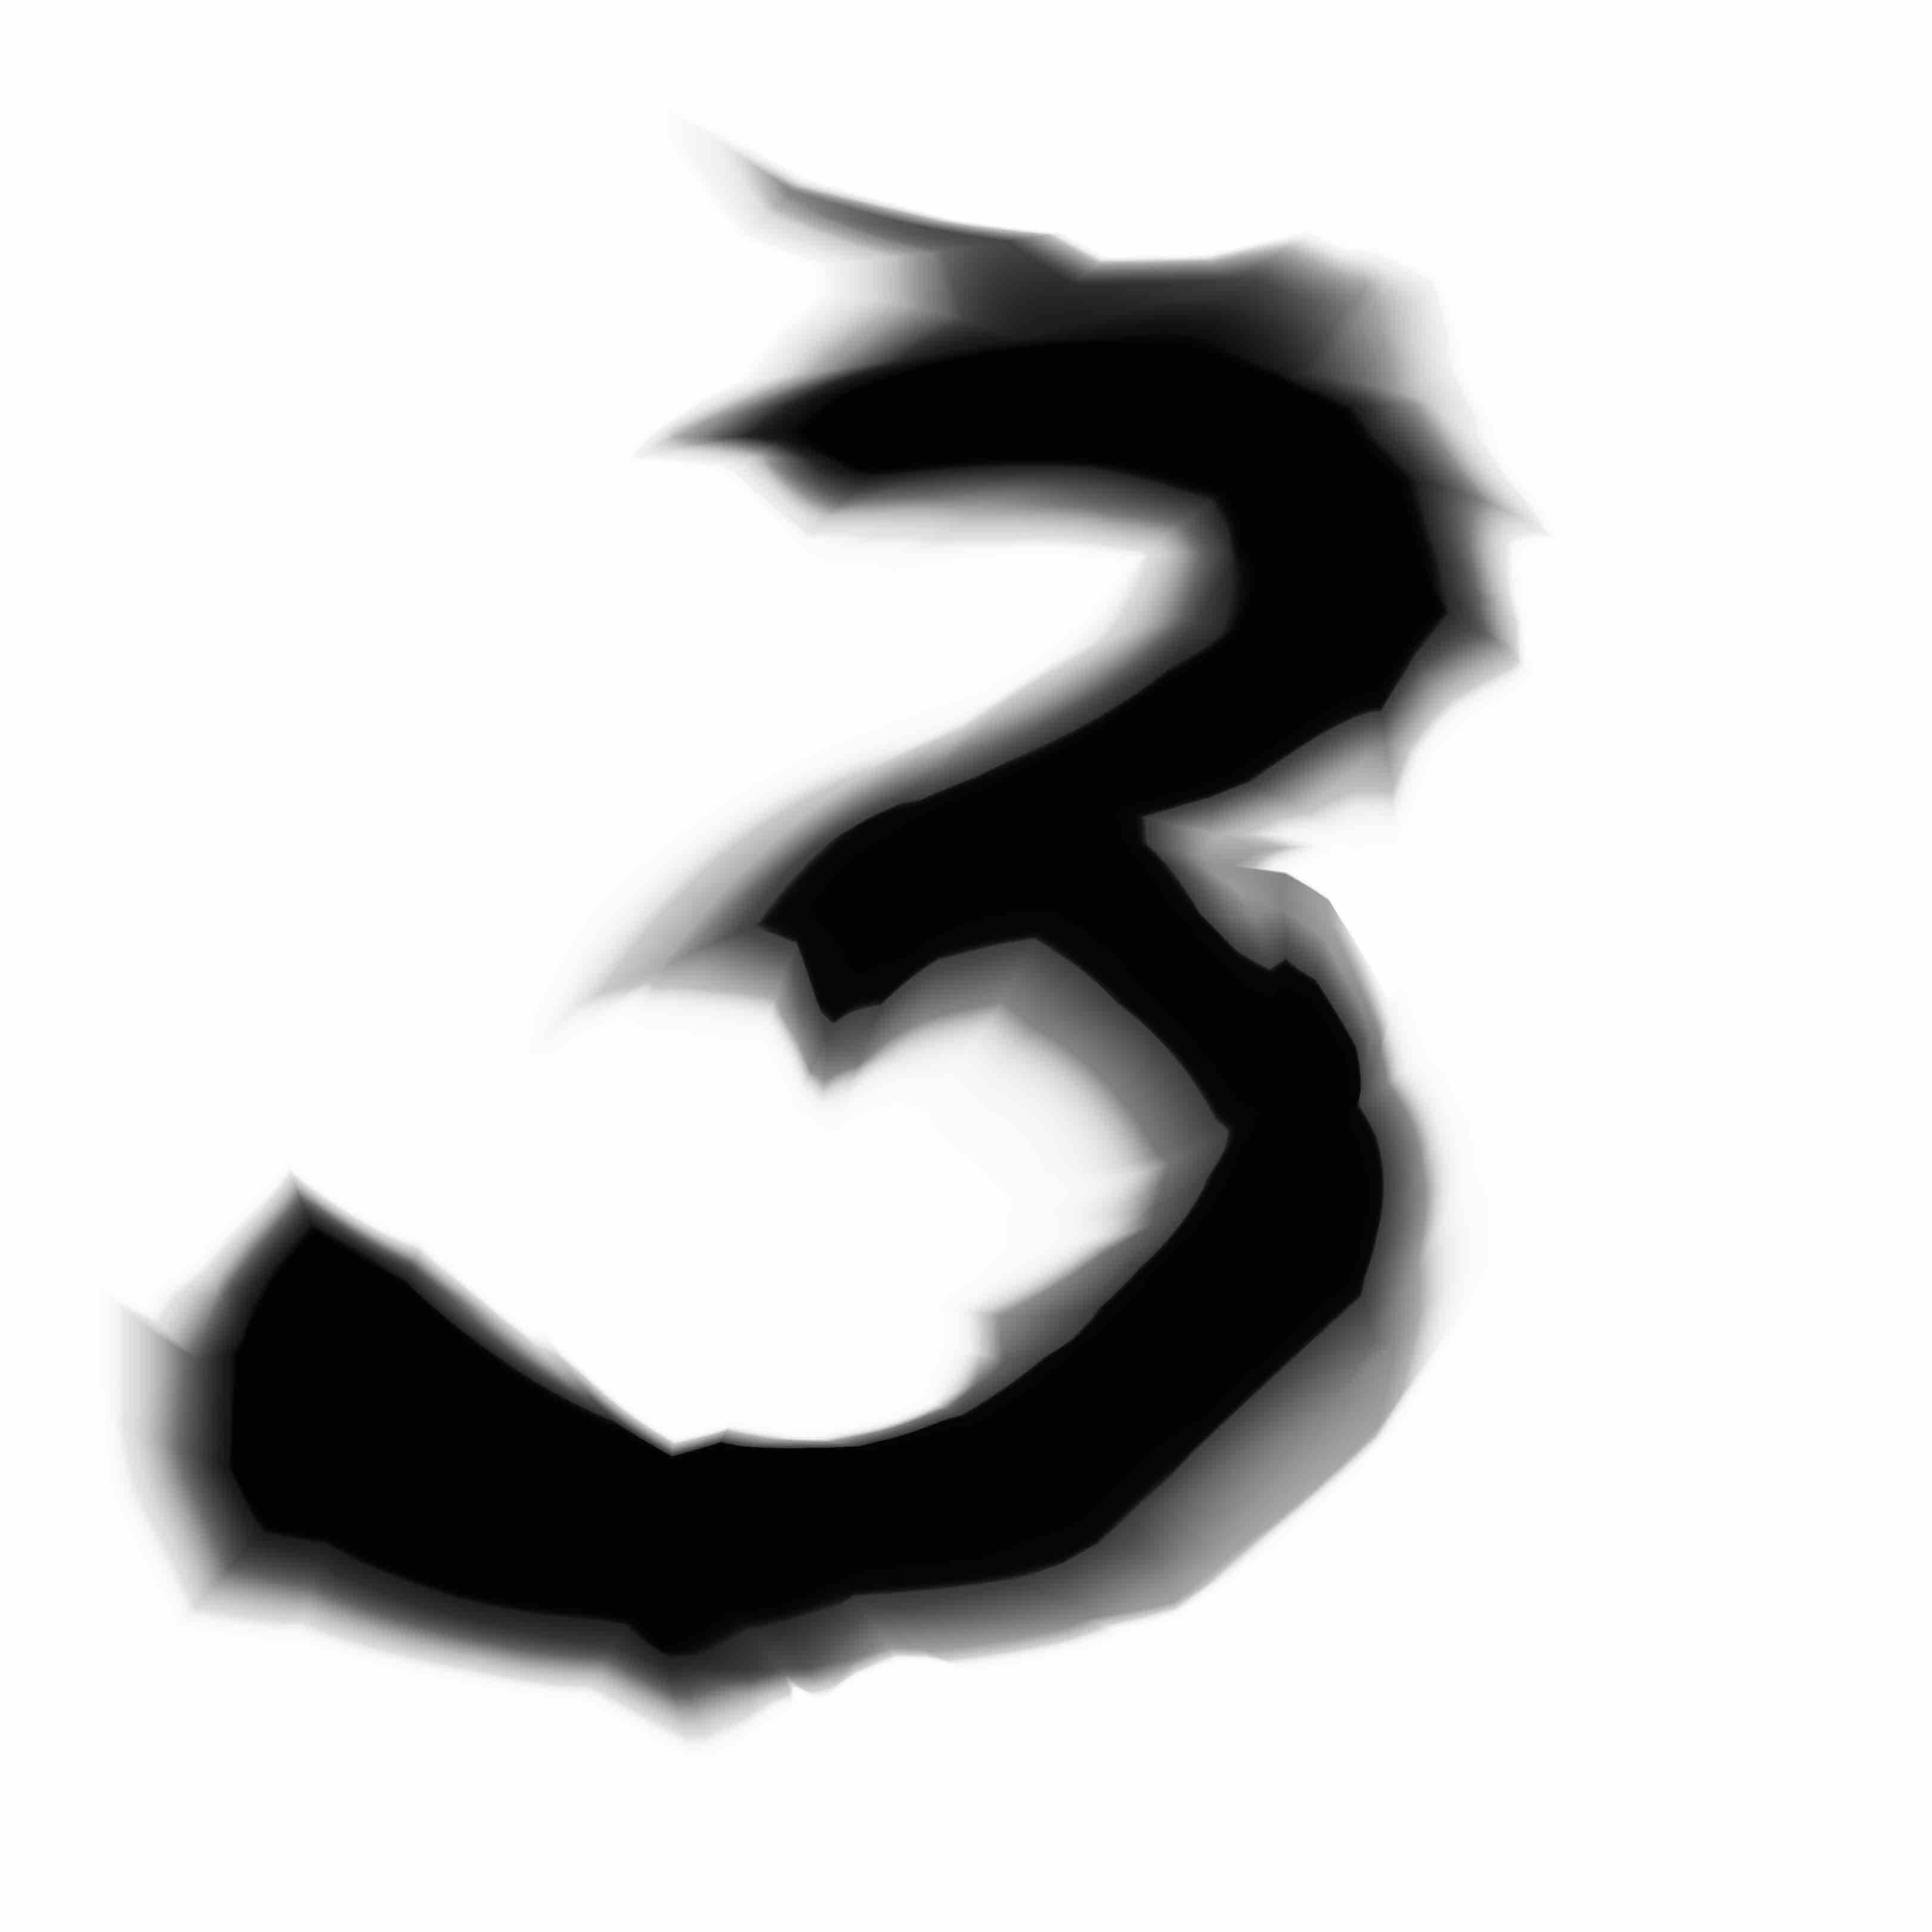
\includegraphics[width=.9\textwidth]{images/three.jpeg}};
		\draw[black, thick] (9.5,2) rectangle (10.5,3);				
		
\end{tikzpicture}

\end{center}
        % \vspace{-0.4in}
        \caption{\small{AE approach (and then train a classifier on top of this hidden representation) }}
    \end{figure}
   
    \end{overlayarea}
  \end{columns}
\end{frame}


\begin{frame}
    \begin{block}{}
        We will now see a way of visualizing AEs and use this visualization to compare different AEs
    \end{block}
\end{frame}

\begin{frame}
  \begin{columns}
    \column{0.4\textwidth}
    \begin{overlayarea}{\textwidth}{\textheight}
        \begin{figure}
            % \tikzstyle{input_neuron}=[circle,draw=red!50,fill=red!10,thick,minimum size=6mm]
\tikzstyle{hidden_neuron}=[circle,draw=blue!50,fill=cyan!10,thick,minimum size=6mm]
\tikzstyle{output_neuron}=[circle,draw=green!50,fill=green!10,thick,minimum size=6mm]
\tikzstyle{cpy_neuron}=[circle,draw=blue!50,fill=blue!50,thick,minimum size=6mm]
\tikzstyle{input}=[circle,draw=black!50,fill=black!20,thick,minimum size=6mm]

\begin{center}
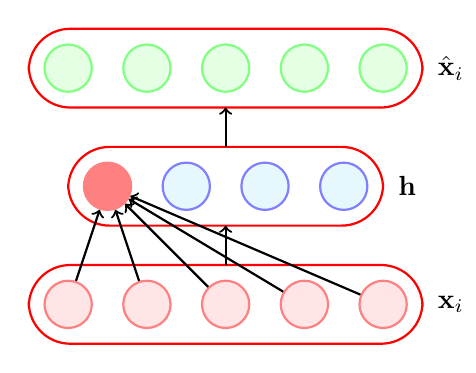
\begin{tikzpicture}

\node [input_neuron] (neuron01) at (6.5,4.5) {};
\node [input_neuron] (neuron02) at (7.5,4.5){};
\node [input_neuron] (neuron03) at (8.5,4.5) {};
\node [input_neuron] (neuron04) at (9.5,4.5) {};
\node [input_neuron] (neuron05) at (10.5,4.5) {};
\node [cpy_neuron] (neuron51) at (7,6) {} ;
\node [hidden_neuron] (neuron52) at (8,6)  {};
\node [hidden_neuron] (neuron53) at (9,6)  {};
\node [hidden_neuron] (neuron54) at (10,6)  {};

\node [output_neuron] (neuron11) at (6.5,7.5)  {};
\node [output_neuron] (neuron12) at (7.5,7.5)  {};
\node [output_neuron] (neuron13) at (8.5,7.5)  {};
\node [output_neuron] (neuron14) at (9.5,7.5)  {};
\node [output_neuron] (neuron15) at (10.5,7.5)  {};

\node[text width=0.01cm] at (11.2,4.5) {$\textbf{x}_i$};
\node[text width=0.01cm] at (10.7,6) {$\textbf{h}$};
\node[text width=0.01cm] at (11.2,7.5) {$\hat{\textbf{x}}_i$};

%\node[] at (8.5,3.2) {AE approach};

\draw[red!100,thick,solid,rounded corners=15pt] (6,4) rectangle (11,5);
\draw[red!100,thick,solid,rounded corners=15pt] (6.5,5.5) rectangle (10.5,6.5);
\draw[red!100,thick,solid,rounded corners=15pt] (6,7) rectangle (11,8);
\draw[thick,->](neuron01) -- (neuron51);
\draw[thick,->](neuron02) -- (neuron51);
\draw[thick,->](neuron03) -- (neuron51);
\draw[thick,->](neuron04) -- (neuron51);
\draw[thick,->](neuron05) -- (neuron51);

\draw[thick,->] (8.5,5) -- (8.5,5.5);

\draw[thick,->] (8.5,6.5) -- (8.5,7);



\end{tikzpicture}
\end{center}

            \tikzstyle{input_neuron}=[circle,draw=red!50,fill=red!10,thick,minimum size=6mm]
\tikzstyle{hidden_neuron}=[circle,draw=blue!50,fill=cyan!10,thick,minimum size=6mm]
\tikzstyle{output_neuron}=[circle,draw=green!50,fill=green!10,thick,minimum size=6mm]
\tikzstyle{cpy_neuron}=[circle,draw=blue!50,fill=blue!50,thick,minimum size=6mm]
\tikzstyle{input}=[circle,draw=black!50,fill=black!20,thick,minimum size=6mm]

\begin{center}
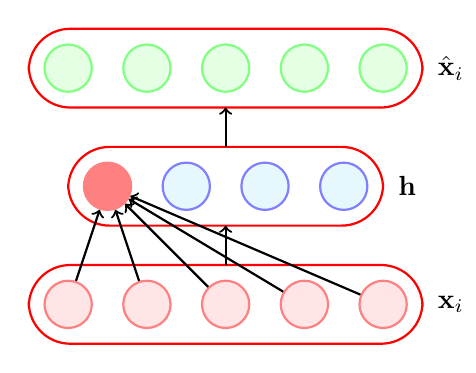
\begin{tikzpicture}

\node [input_neuron] (neuron01) at (6.5,4.5) {};
\node [input_neuron] (neuron02) at (7.5,4.5){};
\node [input_neuron] (neuron03) at (8.5,4.5) {};
\node [input_neuron] (neuron04) at (9.5,4.5) {};
\node [input_neuron] (neuron05) at (10.5,4.5) {};
\node [cpy_neuron] (neuron51) at (7,6) {} ;
\node [hidden_neuron] (neuron52) at (8,6)  {};
\node [hidden_neuron] (neuron53) at (9,6)  {};
\node [hidden_neuron] (neuron54) at (10,6)  {};

\node [output_neuron] (neuron11) at (6.5,7.5)  {};
\node [output_neuron] (neuron12) at (7.5,7.5)  {};
\node [output_neuron] (neuron13) at (8.5,7.5)  {};
\node [output_neuron] (neuron14) at (9.5,7.5)  {};
\node [output_neuron] (neuron15) at (10.5,7.5)  {};

\node[text width=0.01cm] at (11.2,4.5) {$\textbf{x}_i$};
\node[text width=0.01cm] at (10.7,6) {$\textbf{h}$};
\node[text width=0.01cm] at (11.2,7.5) {$\hat{\textbf{x}}_i$};

%\node[] at (8.5,3.2) {AE approach};

\draw[red!100,thick,solid,rounded corners=15pt] (6,4) rectangle (11,5);
\draw[red!100,thick,solid,rounded corners=15pt] (6.5,5.5) rectangle (10.5,6.5);
\draw[red!100,thick,solid,rounded corners=15pt] (6,7) rectangle (11,8);
\draw[thick,->](neuron01) -- (neuron51);
\draw[thick,->](neuron02) -- (neuron51);
\draw[thick,->](neuron03) -- (neuron51);
\draw[thick,->](neuron04) -- (neuron51);
\draw[thick,->](neuron05) -- (neuron51);

\draw[thick,->] (8.5,5) -- (8.5,5.5);

\draw[thick,->] (8.5,6.5) -- (8.5,7);



\end{tikzpicture}
\end{center}

            % \vspace{-1.5cm}
        \end{figure}

    \footnotesize{
    \onslide<5->{
    \begin{block}{}
    \begin{align*}
        \underset{\textbf{x}_i}{\max} \hspace{0.1in} & \{W_{1}^{T}\textbf{x}_{i}\}\\
         s.t.\hspace{0.1in}  ||\textbf{x}_{i}||^{2} &= \textbf{x}_{i}^{T}\textbf{x}_{i} = 1\\
        \onslide<6->{\text{Solution:}\hspace{0.1in}  \textbf{x}_{i} &= \frac{W_{1}}{\sqrt{W_1^TW_1}}}                             
    \end{align*}
    \end{block}}}


    %$\underset{x}{\arg \max} ~ W^{T}*x ~ s.t. ~ \|{x}\|^2  =  x^T*x = 1$ \\

    %$Solution: x = \frac{W_{1}}{\sqrt{W_1^{T}W_{1}}}$

    \end{overlayarea}

    \column{0.6\textwidth}
    \begin{overlayarea}{\textwidth}{\textheight}
        \only <1-> {
            \begin{itemize}\justifying
                  \item <1-> We can think of each neuron as a filter which will fire (or get maximally) activated for a certain input configuration $\textbf{x}_{i}$ 
                  \item <2-> For example, \\
                     \[\textbf{h}_{1} = \sigma(W_{1}^{T}\textbf{x}_{i}) ~ [ignoring ~ bias ~ b]\]
                     Where $W_{1}$ is the trained vector of weights connecting the input to the first hidden neuron 
                  \item <3-> What values of $\textbf{x}_i$ will cause $\textbf{h}_1$ to be maximum (or maximally activated)
                  \item <4-> Suppose we assume that our inputs are normalized so that $\|{\textbf{x}_i}\| = 1$      
            \end{itemize}
        }
    \end{overlayarea}
  \end{columns}
\end{frame}


\begin{frame}
  \begin{columns}
    \column{0.4\textwidth}
    \begin{overlayarea}{\textwidth}{\textheight}
        \begin{figure}
            % \tikzstyle{input_neuron}=[circle,draw=red!50,fill=red!10,thick,minimum size=6mm]
\tikzstyle{hidden_neuron}=[circle,draw=blue!50,fill=cyan!10,thick,minimum size=6mm]
\tikzstyle{output_neuron}=[circle,draw=green!50,fill=green!10,thick,minimum size=6mm]
\tikzstyle{cpy_neuron}=[circle,draw=blue!50,fill=blue!50,thick,minimum size=6mm]
\tikzstyle{input}=[circle,draw=black!50,fill=black!20,thick,minimum size=6mm]

\begin{center}
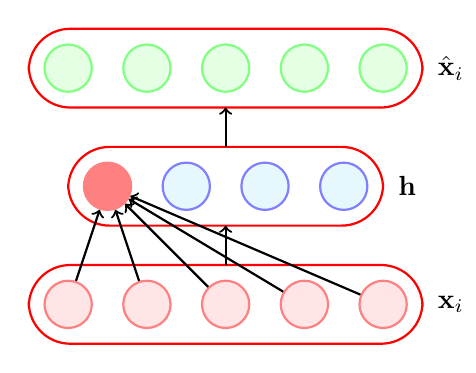
\begin{tikzpicture}

\node [input_neuron] (neuron01) at (6.5,4.5) {};
\node [input_neuron] (neuron02) at (7.5,4.5){};
\node [input_neuron] (neuron03) at (8.5,4.5) {};
\node [input_neuron] (neuron04) at (9.5,4.5) {};
\node [input_neuron] (neuron05) at (10.5,4.5) {};
\node [cpy_neuron] (neuron51) at (7,6) {} ;
\node [hidden_neuron] (neuron52) at (8,6)  {};
\node [hidden_neuron] (neuron53) at (9,6)  {};
\node [hidden_neuron] (neuron54) at (10,6)  {};

\node [output_neuron] (neuron11) at (6.5,7.5)  {};
\node [output_neuron] (neuron12) at (7.5,7.5)  {};
\node [output_neuron] (neuron13) at (8.5,7.5)  {};
\node [output_neuron] (neuron14) at (9.5,7.5)  {};
\node [output_neuron] (neuron15) at (10.5,7.5)  {};

\node[text width=0.01cm] at (11.2,4.5) {$\textbf{x}_i$};
\node[text width=0.01cm] at (10.7,6) {$\textbf{h}$};
\node[text width=0.01cm] at (11.2,7.5) {$\hat{\textbf{x}}_i$};

%\node[] at (8.5,3.2) {AE approach};

\draw[red!100,thick,solid,rounded corners=15pt] (6,4) rectangle (11,5);
\draw[red!100,thick,solid,rounded corners=15pt] (6.5,5.5) rectangle (10.5,6.5);
\draw[red!100,thick,solid,rounded corners=15pt] (6,7) rectangle (11,8);
\draw[thick,->](neuron01) -- (neuron51);
\draw[thick,->](neuron02) -- (neuron51);
\draw[thick,->](neuron03) -- (neuron51);
\draw[thick,->](neuron04) -- (neuron51);
\draw[thick,->](neuron05) -- (neuron51);

\draw[thick,->] (8.5,5) -- (8.5,5.5);

\draw[thick,->] (8.5,6.5) -- (8.5,7);



\end{tikzpicture}
\end{center}

            \tikzstyle{input_neuron}=[circle,draw=red!50,fill=red!10,thick,minimum size=6mm]
\tikzstyle{hidden_neuron}=[circle,draw=blue!50,fill=cyan!10,thick,minimum size=6mm]
\tikzstyle{output_neuron}=[circle,draw=green!50,fill=green!10,thick,minimum size=6mm]
\tikzstyle{cpy_neuron}=[circle,draw=blue!50,fill=blue!50,thick,minimum size=6mm]
\tikzstyle{input}=[circle,draw=black!50,fill=black!20,thick,minimum size=6mm]

\begin{center}
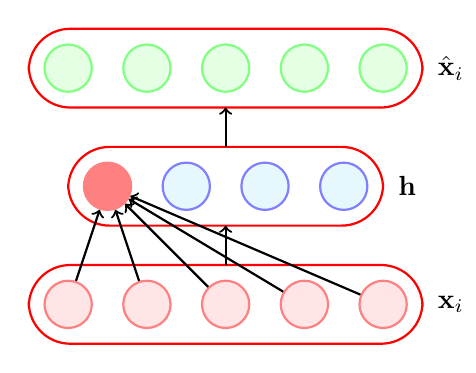
\begin{tikzpicture}

\node [input_neuron] (neuron01) at (6.5,4.5) {};
\node [input_neuron] (neuron02) at (7.5,4.5){};
\node [input_neuron] (neuron03) at (8.5,4.5) {};
\node [input_neuron] (neuron04) at (9.5,4.5) {};
\node [input_neuron] (neuron05) at (10.5,4.5) {};
\node [cpy_neuron] (neuron51) at (7,6) {} ;
\node [hidden_neuron] (neuron52) at (8,6)  {};
\node [hidden_neuron] (neuron53) at (9,6)  {};
\node [hidden_neuron] (neuron54) at (10,6)  {};

\node [output_neuron] (neuron11) at (6.5,7.5)  {};
\node [output_neuron] (neuron12) at (7.5,7.5)  {};
\node [output_neuron] (neuron13) at (8.5,7.5)  {};
\node [output_neuron] (neuron14) at (9.5,7.5)  {};
\node [output_neuron] (neuron15) at (10.5,7.5)  {};

\node[text width=0.01cm] at (11.2,4.5) {$\textbf{x}_i$};
\node[text width=0.01cm] at (10.7,6) {$\textbf{h}$};
\node[text width=0.01cm] at (11.2,7.5) {$\hat{\textbf{x}}_i$};

%\node[] at (8.5,3.2) {AE approach};

\draw[red!100,thick,solid,rounded corners=15pt] (6,4) rectangle (11,5);
\draw[red!100,thick,solid,rounded corners=15pt] (6.5,5.5) rectangle (10.5,6.5);
\draw[red!100,thick,solid,rounded corners=15pt] (6,7) rectangle (11,8);
\draw[thick,->](neuron01) -- (neuron51);
\draw[thick,->](neuron02) -- (neuron51);
\draw[thick,->](neuron03) -- (neuron51);
\draw[thick,->](neuron04) -- (neuron51);
\draw[thick,->](neuron05) -- (neuron51);

\draw[thick,->] (8.5,5) -- (8.5,5.5);

\draw[thick,->] (8.5,6.5) -- (8.5,7);



\end{tikzpicture}
\end{center}

            % \vspace{-1.5cm}
        \end{figure}

    \footnotesize{
    \begin{block}{}
    \begin{align*}
        \underset{\textbf{x}_i}{\max} \hspace{0.1in} & \{W_{1}^{T}\textbf{x}_{i}\}\\
         s.t.\hspace{0.1in}  ||\textbf{x}_i ||^{2} &= \textbf{x}_{i}^{T}\textbf{x}_{i} = 1\\
        \text{Solution:}\hspace{0.1in}  \textbf{x}_{i} &= \frac{W_{1}}{\sqrt{W_1^TW_1}}                               
    \end{align*}
    \end{block}}
    \end{overlayarea}

    \column{0.6\textwidth}
    \begin{overlayarea}{\textwidth}{\textheight}
        \begin{itemize}\justifying
            \item<1-> Thus the inputs \\
             \[ \textbf{x}_{i} =  \frac{W_{1}}{\sqrt{W_1^{T}W_{1}}}, \frac{W_{2}}{\sqrt{W_2^{T}W_{2}}}, \dots \frac{W_{n}}{\sqrt{W_n^{T}W_{n}}}  \]
            will respectively cause hidden neurons $1$ to $n$ to maximally fire    
        
            \item<2-> Let us plot these images ($\textbf{x}_{i}$'s) which maximally activate the first $k$ neurons  of the hidden representations learned by a vanilla autoencoder and different denoising autoencoders
   
            \item<3-> These $\textbf{x}_{i}$'s are computed by the above formula using the weights $(W_{1}, W_{2} \dots W_{k})$ learned by the respective autoencoders
        \end{itemize}
    \end{overlayarea}
  \end{columns}
\end{frame}

\begin{frame}
    \begin{figure}
    \minipage{0.25\textwidth}
        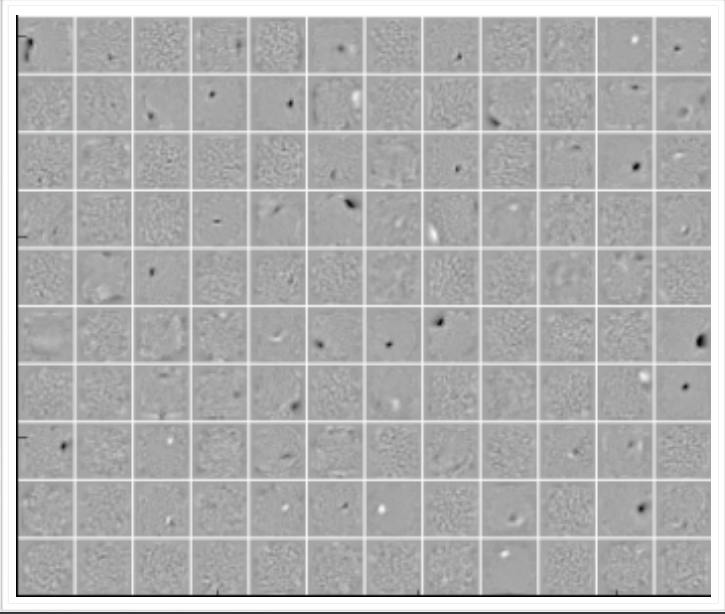
\includegraphics[width=\linewidth,height=3cm]{images/cross-entropy-loss.png}
        \label{fig:awesome_image1}
        \caption{Vanilla AE (No noise)}
    \endminipage\hfill
    \minipage{0.25\textwidth}
        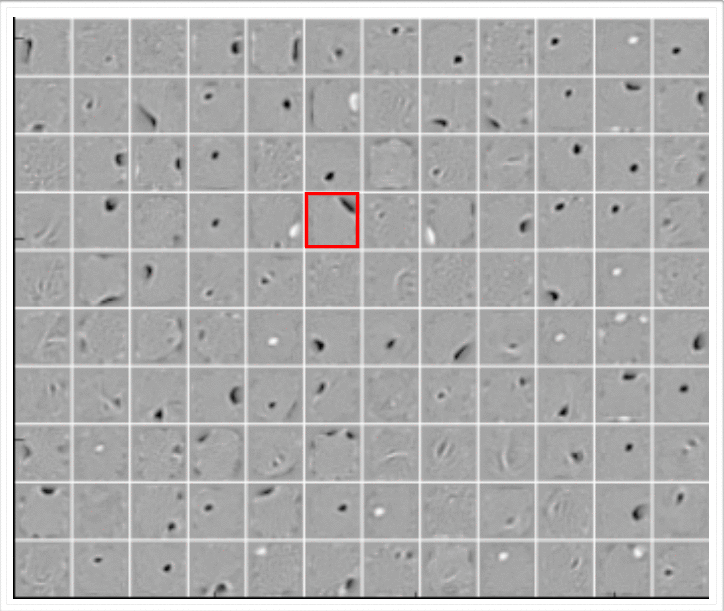
\includegraphics[width=\linewidth, height=3cm]{images/25_edited2.png}
        \label{fig:awesome_image2}
        \caption{25\% Denoising AE (q=0.25)}
    \endminipage\hfill
    \minipage{0.25\textwidth}%
        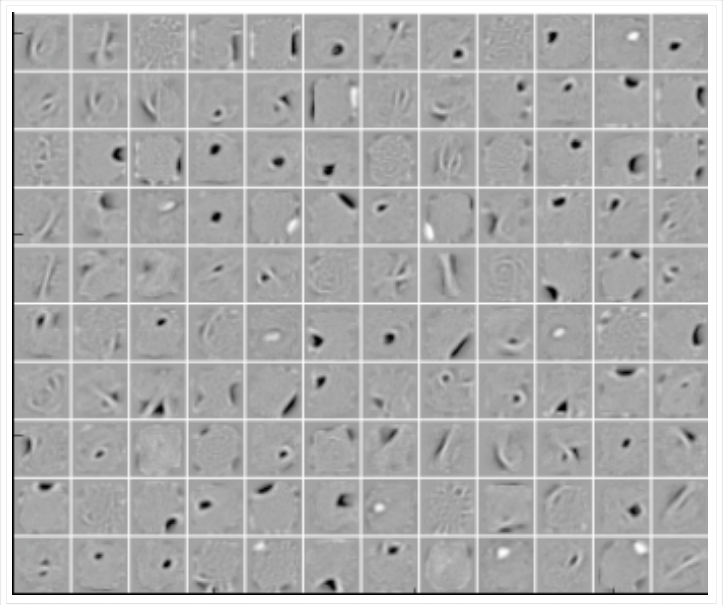
\includegraphics[width=\linewidth,height=3cm]{images/50.png}
        \label{fig:awesome_image3}
        \caption{50\% Denoising AE (q=0.5)}
    \endminipage
    \end{figure}

    \begin{itemize}\justifying
        \item<1-> The vanilla AE does not learn many meaningful patterns
        \item<2-> The hidden neurons of the denoising AEs seem to act like pen-stroke detectors (for example, in the highlighted neuron the black region is a stroke that you would expect in a '0' or a '2' or a '3' or a '8' or a '9')  
        \item<3-> As the noise increases the filters become more wide because the neuron has to rely on more adjacent pixels to feel confident about a stroke
    \end{itemize}
\end{frame}

\begin{frame}

  \begin{columns}
    \column{0.4\textwidth}
        \begin{overlayarea}{\textwidth}{\textheight}
            % \tikzstyle{input_neuron}=[circle,draw=red!50,fill=red!10,thick,minimum size=6mm]
\tikzstyle{hidden_neuron}=[circle,draw=blue!50,fill=cyan!10,thick,minimum size=6mm]
\tikzstyle{output_neuron}=[circle,draw=green!50,fill=green!10,thick,minimum size=6mm]
\tikzstyle{cpy_neuron}=[circle,draw=red!50,fill=red!50,thick,minimum size=6mm]
\tikzstyle{input}=[circle,draw=black!50,fill=black!20,thick,minimum size=6mm]

\begin{center}
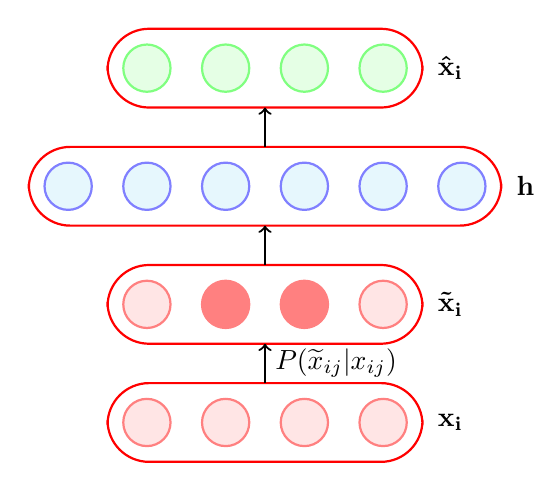
\begin{tikzpicture}

\node [input_neuron] (neuron001) at (8.5,3) {};
\node [input_neuron] (neuron002) at (9.5,3){};
\node [input_neuron] (neuron003) at (10.5,3) {};
\node [input_neuron] (neuron004) at (11.5,3) {};

\node [input_neuron] (neuron01) at (8.5,4.5) {};
\node [cpy_neuron] (neuron02) at (9.5,4.5){};
\node [cpy_neuron] (neuron03) at (10.5,4.5) {};
\node [input_neuron] (neuron04) at (11.5,4.5) {};

\node [hidden_neuron] (neuron51) at (7.5,6) {} ;
\node [hidden_neuron] (neuron52) at (8.5,6)  {};
\node [hidden_neuron] (neuron53) at (9.5,6)  {};
\node [hidden_neuron] (neuron54) at (10.5,6)  {};
\node [hidden_neuron] (neuron55) at (11.5,6)  {};
\node [hidden_neuron] (neuron56) at (12.5,6)  {};

\node [output_neuron] (neuron11) at (8.5,7.5)  {};
\node [output_neuron] (neuron12) at (9.5,7.5)  {};
\node [output_neuron] (neuron13) at (10.5,7.5)  {};
\node [output_neuron] (neuron14) at (11.5,7.5)  {};

\node[text width=0.01cm] at (12.2,3) {$\mathbf{\textbf{x}_i}$};
\node[text width=0.01cm] at (12.2,4.5) {$\mathbf{\tilde{\textbf{x}}_i}$};
\node[text width=0.01cm] at (13.2,6) {$\mathbf{h}$};
\node[text width=0.01cm] at (12.2,7.5) {$\mathbf{\hat{x}_{i}}$};

\draw[red!100,thick,solid,rounded corners=15pt] (8,2.5) rectangle (12,3.5);
\draw[red!100,thick,solid,rounded corners=15pt] (8,4) rectangle (12,5);
\draw[red!100,thick,solid,rounded corners=15pt] (7,5.5) rectangle (13,6.5);
\draw[red!100,thick,solid,rounded corners=15pt] (8,7) rectangle (12,8);

\draw[thick,->] (10,3.5) -- (10,4) node [pos=0.5,right] {$P(\widetilde{x}_{ij}|x_{ij})$};

\draw[thick,->] (10,5) -- (10,5.5);

\draw[thick,->] (10,6.5) -- (10,7);

\end{tikzpicture}
\end{center}
            \tikzstyle{input_neuron}=[circle,draw=red!50,fill=red!10,thick,minimum size=6mm]
\tikzstyle{hidden_neuron}=[circle,draw=blue!50,fill=cyan!10,thick,minimum size=6mm]
\tikzstyle{output_neuron}=[circle,draw=green!50,fill=green!10,thick,minimum size=6mm]
\tikzstyle{cpy_neuron}=[circle,draw=red!50,fill=red!50,thick,minimum size=6mm]
\tikzstyle{input}=[circle,draw=black!50,fill=black!20,thick,minimum size=6mm]

\begin{center}
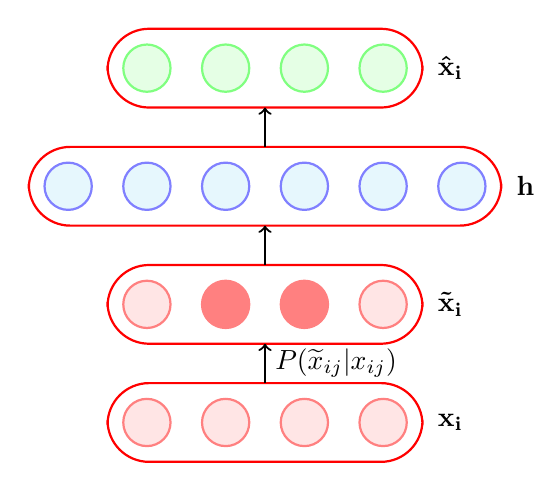
\begin{tikzpicture}

\node [input_neuron] (neuron001) at (8.5,3) {};
\node [input_neuron] (neuron002) at (9.5,3){};
\node [input_neuron] (neuron003) at (10.5,3) {};
\node [input_neuron] (neuron004) at (11.5,3) {};

\node [input_neuron] (neuron01) at (8.5,4.5) {};
\node [cpy_neuron] (neuron02) at (9.5,4.5){};
\node [cpy_neuron] (neuron03) at (10.5,4.5) {};
\node [input_neuron] (neuron04) at (11.5,4.5) {};

\node [hidden_neuron] (neuron51) at (7.5,6) {} ;
\node [hidden_neuron] (neuron52) at (8.5,6)  {};
\node [hidden_neuron] (neuron53) at (9.5,6)  {};
\node [hidden_neuron] (neuron54) at (10.5,6)  {};
\node [hidden_neuron] (neuron55) at (11.5,6)  {};
\node [hidden_neuron] (neuron56) at (12.5,6)  {};

\node [output_neuron] (neuron11) at (8.5,7.5)  {};
\node [output_neuron] (neuron12) at (9.5,7.5)  {};
\node [output_neuron] (neuron13) at (10.5,7.5)  {};
\node [output_neuron] (neuron14) at (11.5,7.5)  {};

\node[text width=0.01cm] at (12.2,3) {$\mathbf{\textbf{x}_i}$};
\node[text width=0.01cm] at (12.2,4.5) {$\mathbf{\tilde{\textbf{x}}_i}$};
\node[text width=0.01cm] at (13.2,6) {$\mathbf{h}$};
\node[text width=0.01cm] at (12.2,7.5) {$\mathbf{\hat{x}_{i}}$};

\draw[red!100,thick,solid,rounded corners=15pt] (8,2.5) rectangle (12,3.5);
\draw[red!100,thick,solid,rounded corners=15pt] (8,4) rectangle (12,5);
\draw[red!100,thick,solid,rounded corners=15pt] (7,5.5) rectangle (13,6.5);
\draw[red!100,thick,solid,rounded corners=15pt] (8,7) rectangle (12,8);

\draw[thick,->] (10,3.5) -- (10,4) node [pos=0.5,right] {$P(\widetilde{x}_{ij}|x_{ij})$};

\draw[thick,->] (10,5) -- (10,5.5);

\draw[thick,->] (10,6.5) -- (10,7);

\end{tikzpicture}
\end{center}
        \end{overlayarea}

    \column{0.6\textwidth}
    \begin{overlayarea}{\textwidth}{\textheight}
        \begin{itemize}\justifying
            \item<1-> We saw one form of $P(\widetilde{x}_{ij} | x_{ij})$ which flips a fraction $q$ of the inputs to zero
            \item<2-> Another way of corrupting the inputs is to add a Gaussian noise to the input \\
            \[\widetilde{x}_{ij} = x_{ij} + \mathscr{N}(0,1)\]
            \item<3-> We will now use such a denoising AE on a different dataset and see their performance
        \end{itemize}
    \end{overlayarea}
  \end{columns}
\end{frame}

\begin{frame}
    \begin{figure}
    \minipage{0.25\textwidth}
        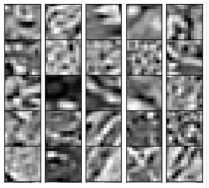
\includegraphics[width=\linewidth]{images/data.png}
        \label{fig:awesome_image1}
        \caption{Data}
    \endminipage\hfill
    \minipage{0.25\textwidth}
        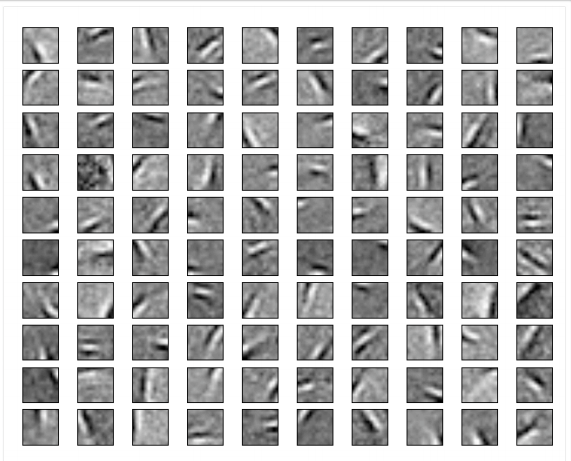
\includegraphics[width=\linewidth]{images/ae-filters.png}
        \label{fig:awesome_image2}
        \caption{AE filters}
    \endminipage\hfill
    \minipage{0.25\textwidth}%
        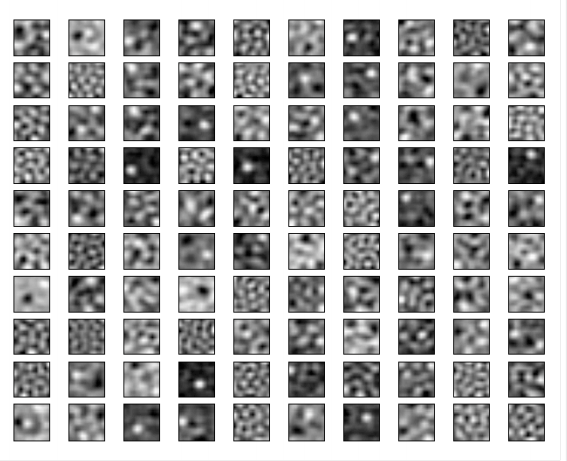
\includegraphics[width=\linewidth]{images/weight-decay.png}
        \label{fig:awesome_image3}
        \caption{Weight decay filters}
    \endminipage
    \label{pics:blablabla}
    \end{figure}

    \begin{itemize}\justifying
        \item<1-> The hidden neurons essentially behave like edge detectors
        \item<2-> PCA does not give such edge detectors
        % \item<3-> Also note that even though the noise process (adding Gaussian noise) is similar to weight decay penalty the results are very different (in particular with weight decay we do not see any meaningful patterns)   
    \end{itemize}
\end{frame}

% Slide 39 Module 4 ends
